\documentclass[]{VUMIFTemplateClass}

\usepackage{indentfirst}
\usepackage{amsmath, amsthm, amssymb, amsfonts}
\usepackage{mathtools}
\usepackage{physics}
\usepackage{graphicx}
\usepackage{verbatim}
\usepackage[hidelinks]{hyperref}
\usepackage{color,algorithm,algorithmic}
\usepackage[nottoc]{tocbibind}
\usepackage{tocloft}


\usepackage{titlesec}

\usepackage{biblatex}
\bibliography{bibliography}
%% norint pakeisti bibliografijos šaltinių numeravimą (skaitiniu arba raidiniu), pakeitimus atlikti VUMIFTemplateClass.cls 150 eilutėje

\usepackage{longtable}
\usepackage{booktabs}

\usepackage{gensymb}
\usepackage{acro}
\usepackage{tikz}
\usetikzlibrary{decorations.pathreplacing}
\usepackage{amssymb,amsthm}
\usepackage[version=4]{mhchem}

\newcommand{\sectionbreak}{\clearpage}

\makeatletter
\renewcommand{\fnum@algorithm}{\thealgorithm}
\makeatother
\renewcommand\thealgorithm{\arabic{algorithm} algoritmas}

% --------------------------- Footnote Refs ----------------------------------

\makeatletter
\newcommand\footnoteref[1]{\protected@xdef\@thefnmark{\ref{#1}}\@footnotemark}
\makeatother

% --------------------------- Math Tools -------------------------------------

\DeclarePairedDelimiter\set\{\}

% Author's MACROS
\newcommand{\EE}{\mathbb{E}\,} % Mean
\newcommand{\ee}{{\mathrm e}}  % nice exponent
\newcommand{\RR}{\mathbb{R}}
\newcommand{\angl}[1]{\textit{(angl. #1)}}
\newcommand{\Angl}[1]{\textit{angl. #1}}
\newcommand{\zr}[1]{(žr. \ref{#1}~pav.)}

\renewcommand\thesubfigure{\thefigure.\alph{subfigure}} % Makes 1.a, 1.b
\captionsetup[subfigure]{labelformat=simple}
\studijuprograma{Programų sistemų} %Studijų programą įrašyti kilmininko linksniu (pavyzdžiui – Programų sistemų, Finansų ir draudimų matematikos ir t. t.)
\darbotipas{Bakalauro baigiamasis darbas} % Bakalauro baigiamasis darbas arba magistro baigiamasis darbas
\darbopavadinimas{Maišymo proceso modeliavimas YAG reakcijose}
\darbopavadinimasantras{Modelling the mixing process in YAG reactions}
\autorius{Arnas Vaicekauskas}

%Autorių gali būti ir daugiau, tuo atveju, kiekvienas autorius rašomas iš naujos eilutės, ir pridedamas titulinis.tex arba dvigubasTitulinis.tex dokumentuose
%\antrasautorius{Vardas Pavardė} %Jei toks yra, kitu atveju ištrinti

\vadovas{asist. dr. Rokas Astrauskas}
\recenzentas{prof. dr. (HP) Romas Baronas} %Jei toks yra žinomas, kitu atveju ištrinti
% \moksliniskonsultantas{pedagoginis/mokslinis vardas Vardas Pavardė} %Jei toks yra žinomas, kitu atveju ištrinti

\begin{document}

\selectlanguage{lithuanian}
\onehalfspacing
\begin{titlepage}
\vskip 20pt
\begin{center}

\includegraphics[scale=0.55]{images/MIF.png}
\end{center}

\makeatletter

\vskip 20pt
\centerline{\bf \large \textbf{VILNIAUS UNIVERSITETAS}}
\vskip 10pt
\centerline{\large \textbf{MATEMATIKOS IR INFORMATIKOS FAKULTETAS}}
\vskip 10pt
\centerline{\large \textbf{\MakeUppercase{\@studijuprograma \space studijų programa}}}

\vskip 80pt
\centerline{\Large \@darbotipas}
\vskip 20pt
\begin{center}
    {\bf \LARGE \@darbopavadinimas}
\end{center}
\begin{center}
    {\bf \Large \@darbopavadinimasantras}
\end{center}
\vskip 80pt

\centering{\Large \@autorius}
\@ifundefined{@antrasautorius}{}
{
\vskip 10pt
\centering{\Large \@antrasautorius}
}
\vskip 20pt

\centering{
    \begin{tabular}{rcp{.7\textwidth}}
        {\Large Darbo vadovas} & {\Large :} & {\Large \@vadovas}\\[10pt]
        \@ifundefined{@moksliniskonsultantas}{}
            {
                {\Large Mokslinis konsultantas} & {\Large :} & {\Large \@moksliniskonsultantas}\\[10pt]
            }
        \@ifundefined{@recenzentas}{}
            {
                {\Large Recenzentas} & {\Large :} & {\Large \@recenzentas}\\[10pt]
            }
    \end{tabular}}


\vskip 110pt

\centerline{\large \textbf{Vilnius}}
\centerline{\large \textbf{\the\year{}}}

\makeatother

\newpage
\end{titlepage}
%\newgeometry{top=2cm,bottom=2cm,right=2cm,left=3cm}
\setcounter{page}{2}


%Turinys
\tableofcontents
\onehalfspacing

\sectionnonum{Įvadas}

Itrio aliuminio granatas (YAG) yra kristalinis junginys, pasižymintis išskirtinėmis optinėmis savybėmis. Dėl šių savybių YAG kristalai, legiruoti neodimio jonais, plačiai naudojami kaip lazerių aktyvioji terpė. Tokie lazeriai taikomi įvairiose srityse, įskaitant odontologiją \cite{valentiUseErYAG2021}, pramoninę gamybą \cite{dubeyExperimentalStudyNd2008} ir daugelį kitų.

YAG gali būti sintezuojamas keliais skirtingais būdais, įskaitant kietafazę reakciją, solvoterminį procesą, nusodinimą, purškiamo aerozolio terminį skilimą ir zolio-gelio metodą. Daugelis šių metodų yra chemiškai sudėtingi ir reikalauja specializuotos laboratorinės įrangos. Tarp jų kietafazė reakcija išsiskiria kaip paprasčiausias ir pramoninei gamybai tinkamiausias sintezės būdas \cite{zhangNovelSynthesisYAG2005}. Šios reakcijos metu itrio ir aliuminio oksidai reaguoja aukštoje temperatūroje, susidarant YAG kristalams. Praktikoje šios reakcijos greitį galima padidinti periodiškai maišant reagentus.

Kompiuterinis fizinių bei cheminių procesų modeliavimas yra plačiai taikomas tyrimo metodas, leidžiantis giliau suprasti ir tiksliau prognozuoti tokių procesų eigą bei jų rezultatus. Šis metodas itin naudingas YAG sintezės reakcijų analizėje, kadangi laboratoriniai eksperimentai suteikia ribotas galimybes detaliai ištirti vykstančius mechanizmus. Todėl šiame darbe modeliuosime YAG sintezės reakciją kaip reakcijos-difuzijos sistemą. Nors šis metodas taikomas jau ilgą laiką, jis išlieka aktualus ir šiandien. Matematinį YAG reakcijos modelį pasiūlė Ivanauskas et al. \cite{ivanauskasModellingSolidState2005}, o susijusiuose darbuose \cite{ivanauskasComputationalModellingYAG2009,mackeviciusCloserLookComputer2012} eksperimentiniu būdu nustatytos fizinės modelio konstantos, todėl skaičiavimų rezultatus galima tiksliai palyginti su eksperimentiniais duomenimis. Minėtuose straipsniuose dėmesys skiriamas pačiai YAG sintezės reakcijai ir koeficientų nustatymui ir dėl to reakcija yra modeliuojama labai mažoje fizinėje erdvėje, kurioje telpa vos kelios mikrodalelės. Šiame darbe yra tiriamas maišymo mechanizmo poveikis reakcijai, kuris gali kisti priklausomai nuo fizinės erdvės dydžio, todėl yra reikšminga modeliuoti įvairaus dydžio erdves.

Šią reakciją aprašo trijų netiesinių parabolinių dalinių diferencialinių lygčių sistema, sudaranti reakcijos-difuzijos modelį. Tokiose sistemose analitinis sprendinys paprastai neegzistuoja, todėl jų sprendimui taikomi skaitiniai metodai. Vienas iš dažniausiai naudojamų metodų yra baigtinių elementų metodas (\textit{angl. finite element method, FEM}) - jis leidžia suskaidyti nagrinėjamą sritį į mažesnius elementus ir spręsti diferencialines lygtis kiekviename iš jų. Taip pat gali būti taikomas ribinių elementų metodas (\textit{angl. boundary element method, BEM}), kuris naudoja tik ribinių sąlygų informaciją, todėl yra efektyvus sprendžiant uždavinius su sudėtingomis geometrijomis.

Šiame darbe reakcijos-difuzijos sistemai spręsti taikysime du baigtinių skirtumų metodus (\textit{angl. finite difference method, FDM}). Pirmasis - išreikštinis FTCS metodas (\textit{angl. Forward-Time Centered-Space}), dar žinomas kaip Oilerio integracija. Šis metodas pasižymi paprasta implementacija, tačiau yra sąlyginai stabilus ir nėra itin tikslus. Antrasis metodas - neišreikštinis kintamosios krypties metodas (\textit{angl. alternating direction implicit, ADI}), kuris yra techniškai sudėtingesnis, tačiau nesąlyginai stabilus ir užtikrina didesnį tikslumą \cite{doi:10.1137/0103003}. Nepaisant to, kad ADI metodas sukurtas jau seniai, jis vis dar plačiai naudojamas \cite{gaidamauskaiteComparisonFiniteDifference2007}. Šie skaitiniai metodai detaliai aprašyti literatūroje \cite{pressNumericalRecipes3rd2007,levequeFiniteDifferenceMethods2007}.

Itrio aliuminio granato (YAG) kristalai legiruoti su neodimio arba kitų lantanoidų jonais yra naudojami kaip kietakūnių lazerių aktyviosios terpės dėl savo geidžiamų optinių savybių. Šios medžiagos lazeriai yra dažnai taikomi gamybos ir medicinos srityse \cite{dubeyExperimentalStudyNd2008, valentiUseErYAG2021}. Šiai medžiagai sintezuoti yra žinoma keletas būdų, tačiau kietafazės reakcijos metodas yra lengviausiai pritaikomas pramoninei gamybai \cite{bhattacharyyaMethodsSynthesisY3AI5O122007, zhangNovelSynthesisYAG2005}. Praktikoje, (YAG) sintezė, kietafazės reakcijos metodu, užtrunka mažiausiai kelias valandas priklausomai nuo temperatūros, kurioje vykdomas atkaitinimo procesas \cite{mackeviciusCloserLookComputer2012}. Yra žinoma, kad chemikai bando spartinti šią reakcija periodiškai išmaišydami reagentus.

Ivanauskas et al \cite{ivanauskasModellingSolidState2005} pasiūlė matematinį kietafazės (YAG) reakcijos modelį ir nustatė reakcijos greičio ir difuzijos konstantas prie tam tikrų temperatūrų, tačiau šis modelis nemodeliuoja minėto išmaišymo proceso. Kompiuterinis modelis, apimantis išmaišymo procesą, galėtų padėti efektyviau suprasti kokią įtaką maišymas turi šiam procesui ir jo trukmei. Šiame darbe įgyvendinsime kompiuterinį reakcijos modelį, pateiksime porą skirtingų išmaišymo modelių ir juos integruosime į kompiuterinį modelį. Nagrinėsime modelio teorinį stabilumą ir modelio rezultatų korektiškumą. Pateiksime ir išanalizuosime įvairiai agreguotus modelio rezultatus.

Šio \textbf{darbo tikslas} yra sudaryti kompiuterinę difuzijos-reakcijos sistemą, kuri modeliuotų kietafazę YAG reakciją bei ištirti maišymo modelio poveikį YAG kristalų sintezės spartai modeliuojant reakcija įvairaus dydžio erdvėse. Iškelti darbo uždaviniai:

\begin{enumerate}
  
    \item Sudaryti kompiuterinius YAG reakcijos modelius remiantis baigtinių skirtumų skaitiniais metodais
    \item Patikrinti kompiuterinių modelių rezultatų korektiškumą bei palyginti modelių rezultatus tarpusavyje
    \item Apibrėžti medžiagų maišymo modelius
    \item Integruoti medžiagų maišymo modelius į skaitinius YAG reakcijos modelius
    \item Ištirti kompiuterinių modelių rezultatus įvairaus dydžio erdvėse
\end{enumerate}
\section{YAG reakcijos matematinis modeliavimas}

Šiame darbe yra modeliuojama kietafazė reakcija, kurios metu reaguodami itrio ir aliuminio oksidai sudaro itrio aliuminio granato kristalus arba tiesiog (YAG):
\begin{align*}
  \ce{3Y_2O_3 + 5Al_2O_3 -> 2Y_3Al_5O_12}
\end{align*}

Prieš pradedant reakciją metalų oksidai yra sutrinami iki smulkiagrūdžių miltelių ir maišomi kol susidaro homogeniškas mišinys. Metalų oksidų mišinys yra nuolat kaitinamas aukštesnėje negu 1000\degree C temperatūroje. Tokioje temperatūroje metalų oksidai lydosi ir vyksta medžiagų difuzija, todėl reakcijos produktas formuojasi ties mikrodalelių sienelėmis. Priklausomai nuo pasirinktos temperatūros gali kisti dalelių savybės - dalelių tūris, reakcijos ir difuzijos sparta. Eksperimentiniu būdu išmatuota, kad individualių mikrodalelių turiai prie 1000\degree C siekia $1\mu \text{m}^3$, o prie 1600\degree C temperatūros siekia apie $10\mu\text{m}^3$ \cite{ivanauskasComputationalModellingYAG2009}. Minėtame šaltinyje autoriai taip pat pateikia reakcijos bei difuzijos konstantas prie skirtingų temperatūrų:




\begin{figure}[h]
  \centering
  \includegraphics[width=0.25\linewidth]{images/metal_oxides_mixture.png}
  \caption{Priartinto metalų oksidų mišinio iliustracija \cite{ivanauskasComputationalModellingYAG2009}}
  \label{fig:metal-oxides-mixuter}
\end{figure}

Verta paminėti, kad \ref{fig:metal-oxides-mixuter}-ame pavyzdyje matoma iliustracija nėra iki galo tiksli, yra žinoma, kad mikrodalelės yra išsidėsčiusios glaudžiai.
\cite{ivanauskasModellingSolidState2005} Ivanauskas et al pasiūlė modelį, kuriame mikrodalelės yra laikomos kubo arba kvadrato formos priklausomai nuo dimensijos, kurioje modeliuojama reakciją. Laikoma, kad dalelės erdvėje yra periodiškai pasikartojančios, todėl užtenka modeliuoti mažą sritį, kurioje susiduria skirtingų medžiagų dalelės. 

\begin{figure}[h]
  \centering
  \includegraphics[width=0.75\linewidth]{images/periodic-space.png}
  \caption{Periodiškas reakcijos erdvės modelis, čia dalelės tūris $V=a^3=10\mu m$ \cite{ivanauskasComputationalModellingYAG2009}}
  \label{fig:periodic-space}
\end{figure}

Vykstant reakcijai, chemikai periodiškai ištraukia reagentus iš krosnies, kurioje vyksta reakcija, todėl maišymas vyksta prie daug žemesnės temperatūros. Milteliai yra išmaišomi nepažeidžiant mikrodalelių struktūros - t. y. maišoma taip, kad mikrodalelės neskiltų.
% skyrius apie matematinį modelį

\section{Matematinis modelis}

Šiame darbe yra naudojamas (YAG) reakcijos modelis, kurį pasiūlė Ivanauskas et al \cite{ivanauskasModellingSolidState2005}. Yra žinoma, kad reakcijos produktas yra kristalas ir nedifunduoja, todėl difuzijos dėmens trečioje lygtyje nėra. Šis matematinis modelis yra reakcijos-difuzijos sistema, kuriai spręsti naudojamas išreikštinių baigtinių skirtumų metodas \cite{pressNumericalRecipes3rd2007}. Procesas yra modeliuojamas dviejose dimensijose - stačiakampio srityje.

\begin{subequations} \label{rect}
	\begin{align}
		\frac{\partial c_1}{\partial t} & =-3kc_1c_2+D\left(\frac{\partial^2c_1}{\partial x^2}+\frac{\partial^2c_1}{\partial y^2}\right) \\
		\frac{\partial c_2}{\partial t} & =-5kc_1c_2+D\left(\frac{\partial^2c_2}{\partial x^2}+\frac{\partial^2c_2}{\partial y^2}\right) & (x, y, t)&\in\Omega\times[0, T]\\
		\frac{\partial c_3}{\partial t} & =2kc_1c_2
	\end{align}
\end{subequations}

Čia $c_1,c_2,c_3$ yra medžiagų koncentracija, $t$ - laikas, $T$ - proceso trukmė, $W$ - stačiakampio plotis, $H$ - stačiakampio aukštis,
$D$ - medžiagų $c_1$ ir $c_2$ difuzijos konstanta, $k$ - reakcijos greičio konstanta, $\Omega=(0, W)\times(0, H)$ - stačiakampio sritis, kurioje vyksta reakcija. Srities $\Omega$ kraštinę žymėsime $\partial\Omega$:
\begin{align*}
    \partial\Omega=\{0, W\}\times[0, H]\cup[0, W]\times\{0, H\}
\end{align*}
Šios sistemos modelis yra uždaras - medžiagos neprateka pro stačiakampio srities kraštinę $\partial\Omega$, t.~y. taikoma Neumano kraštinė sąlyga:
\begin{align} \label{general-boundary-cond}
	\nabla c_m(x, y, t)\cdot\vec{n}&=0, & (x, y)&\in\partial\Omega & t&\in[0, T] & m&=1, 2, 3
\end{align}
Čia $\nabla c_m$ yra medžiagos $c_m$ gradientas, o $\vec{n}$ - paviršiaus $\partial\Omega$ normalė. Išskleidus kraštines sąlygas \eqref{general-boundary-cond} dviejose dimensijose gauname:
\begin{equation} \label{boundary-cond}
\begin{aligned}
\begin{split}
    \frac{\partial c_m}{\partial x}\Big|_{x=0}=\frac{\partial c_m}{\partial x}\Big|_{x=W}&=0 & y&\in[0,H] & t&\in[0, T] & m&=1, 2, 3\\
    \frac{\partial c_m}{\partial y}\Big|_{y=0}=\frac{\partial c_m}{\partial y}\Big|_{y=H}&=0 & x&\in[0,W] & t&\in[0, T] & m&=1, 2, 3
\end{split}
\end{aligned}
\end{equation}

\newpage
Ruošiant medžiagas reakcijai yra sudaromas stoichiometrinis medžiagų mišinys, todėl matematiniam modeliui yra taikomos šios pradinės sąlygos:
\begin{equation} \label{intial-cond}
	\begin{aligned}
		c_1(x, y, 0) & = \begin{cases} 3c_0, & \text{jei } (x, y)\in\Omega_1 \\ 0, & \text{kitaip} \end{cases} & \Omega_1&=\big(0, \tfrac{W}{2}\big]\times\big(0, \tfrac{H}{2}\big]\cup\big[\tfrac{W}{2}, W\big)\times\big[\tfrac{H}{2}, H\big)\\
		c_2(x, y, 0) & = \begin{cases} 5c_0, & \text{jei } (x, y)\in\Omega_2 \\ 0, & \text{kitaip} \end{cases} & \Omega_2&=\big(0, \tfrac{W}{2}\big)\times\big(\tfrac{H}{2}, H\big)\cup\big(\tfrac{W}{2}, W\big)\times\big(0, \tfrac{H}{2}\big)\\
		c_3(x, y, 0)&=0 & (x, y)&\in\overline{\Omega}=\Omega\cup\partial\Omega\\.
	\end{aligned}
\end{equation}

Čia $3c_0$ ir $5c_0$ atitinkamai yra medžiagų $c_1$ ir $c_2$ dalelių tankiai.

\begin{figure}[h!]
	\centering
	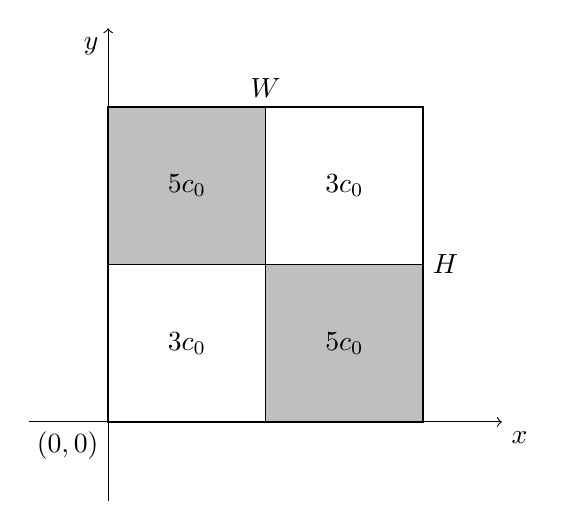
\begin{tikzpicture}[scale=2.0]
		\draw[fill=white] (0,0) rectangle (1,1);
		\draw[fill=white] (1,1) rectangle (2,2);
		\draw[fill=gray!50] (0,1) rectangle (1,2);
		\draw[fill=gray!50] (1,0) rectangle (2,1);

		% Draw the boundary of the square
		\draw[thick] (0,0) rectangle (2,2);

		% Draw axes
		\draw[->] (-0.5, 0) -- (2.5, 0) node[anchor=north west] {$x$};
		\draw[->] (0, -0.5) -- (0, 2.5) node[anchor=north east] {$y$};

		% Mark the origin
		\node[anchor=north east] at (0,0) {$(0, 0)$};

		% Mark the side length
		\draw[-] (2,0) -- (2,2) node[midway, right] {$H$};
		\draw[-] (0,2) -- (2,2) node[midway, above] {$W$};
		\draw (0.5, 1.5) node[anchor=center] {$5c_0$};
		\draw (1.5, 0.5) node[anchor=center] {$5c_0$};
		\draw (1.5, 1.5) node[anchor=center] {$3c_0$};
		\draw (0.5, 0.5) node[anchor=center] {$3c_0$};
	\end{tikzpicture}
	\caption{Sistemos pradinės sąlygos srityje $\Omega$. Tamsesnė spalva žymį sritį $\Omega_2$, o šviesesnė $\Omega_1$}
\end{figure}

\section{Skaitinis modelis}

\subsection{Erdvės diskretizavimas}

Sudarydami tinklelį skaitiniam modeliui, padaliname stačiakampę erdvę $\Omega$ į $N\times M$ taškų, kurie yra nutolę vienas nuo kito fiksuotais atstumais $\Delta x$ ir $\Delta y$ atitinkamomis ašimis. Analogiškai, laiko erdvę $[0, T]$ padalinsime į $\tau + 1$ taškų, kurie vienas nuo kito yra nutolę tolygiais $\Delta t$ atstumais. Apibūdinta diskretų tinklelį galima užrašyti taip:

\begin{align}
    \omega_W&=\{ x_i : x_i = i\Delta x, \quad i=0, 1, \dots, N - 1 \} & \Delta x&=\frac{W}{N-1} \label{meshx}\\
    \omega_H&=\{ y_j : y_j = j\Delta y, \quad j=0, 1, \dots, M - 1 \} & \Delta y&=\frac{H}{M-1} \label{meshy}\\
    \omega_\tau&=\{ t_n : t_n = n\Delta t,\quad n=0, 1, \dots, \tau\} & \Delta t&=\frac{T}{\tau} \label{mesht}\\
	\omega&=\omega_W\times\omega_H\times\omega_\tau \label{mesh}
\end{align}

\begin{figure}[!h]
\centering
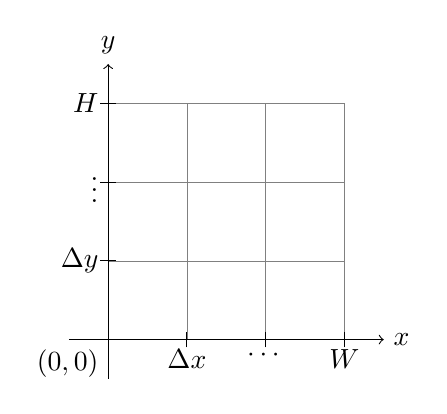
\begin{tikzpicture}
    
% Define the size of the cells
\def\Deltax{1} % Delta x size
\def\Deltay{1} % Delta y size
\def\Xmax{4} % Max X value
\def\Ymax{4} % Max Y value

% Draw the mesh
\foreach \x in {0,1,2} {
    \foreach \y in {0,1,2} {
        \draw[help lines] (\x*\Deltax,\y*\Deltay) grid (\x*\Deltax+\Deltax,\y*\Deltay+\Deltay);
    }
}

\node[below left] at (0,0) {$(0, 0)$};

% Draw axes
\draw[->] (-0.5,0) -- (3.5 *\Deltax,0) node[right] {$x$} ;
\draw[->] (0,-0.5) -- (0,3.5) node[above] {$y$};

% Add tick marks on x-axis with labels
\draw[shift={(1,0)}] (0,-0.1) -- (0,0.1);
\node[below] at (1, 0) {\(\Delta x\)};

\draw[shift={(2,0)}] (0,-0.1) -- (0,0.1);
\node[below] at (2, 0) {$\cdots$};

\draw[shift={(3,0)}] (0,-0.1) -- (0,0.1);
\node[below] at (3, 0) {$W$};

% Add tick marks on y-axis with labels

\draw[shift={(0,1)}] (-0.1,0) -- (0.1,0);
\node[left] at (0, 1) {$\Delta y$};
        
\draw[shift={(0,2)}] (-0.1,0) -- (0.1,0);
\node[left] at (0, 2) {$\vdots$};

\draw[shift={(0,3)}] (-0.1,0) -- (0.1,0);
\node[left] at (0, 3) {$H$};

\end{tikzpicture}
\caption{ Diskretizuota erdvė }
\end{figure}



\newpage
\subsection{Dviejų dimensijų skaitinis modelis}

Remiantis išreikštiniu baigtinių skirtumų metodu pakeisime sistemos \eqref{rect} lygtis su išvestinių aproksimacijomis gautomis skleidžiant išvestines pagal Teiloro eilutę.

\begin{subequations} \label{finite-diffs}
\begin{align}
	\frac{\partial c}{\partial t}\Big|_{x=x_i, y=y_j, t=t_n}&=\frac{c^{n+1}_{i,j}-c^n_{i,j}}{\Delta t} + \mathcal{O}(\Delta t)\\
    \frac{\partial^2c}{\partial x^2}\Big|_{x=x_i, y=y_j, t=t_n}&=\frac{c^n_{i-1,j} - 2c^n_{i,j} + c^n_{i+1,j}}{(\Delta x)^2} + \mathcal{O}((\Delta x)^2)\\
    \frac{\partial^2c}{\partial y^2}\Big|_{x=x_i, y=y_j, t=t_n}&=\frac{c^n_{i,j-1} - 2c^n_{i,j} + c^n_{i,j+1}}{(\Delta y)^2} + \mathcal{O}((\Delta y)^2)
\end{align}
\end{subequations}

Įstate aproksimacijų išraiškas gauname dvimatį skaitini modelį:

\begin{subequations} \label{numerical-eqs}
	\begin{align}
		\frac{c^{n+1}_{1,i,j}-c^n_{1,i,j}}{\Delta t} & =
		-3kc^{n}_{1,i,j}c^{n}_{2,i,j}\notag\\
        & +D\left(\frac{c^n_{1,i-1,j}-2c^n_{1,i,j}+c^n_{1,i+1,j}}{(\Delta x)^2}+\frac{c^n_{1,i,j-1}-2c^n_{1,i,j}+c^n_{1,i,j+1}}{(\Delta y)^2}\right) \\
		\frac{c^{n+1}_{2,i,j}-c^n_{2,i,j}}{\Delta t} & =
		-5kc^{n}_{1,i,j}c^{n}_{2,i,j}\notag\\
        &+D\left(\frac{c^n_{2,i-1,j}-2c^n_{2,i,j}+c^n_{2,i+1,j}}{(\Delta x)^2}+\frac{c^n_{2,i,j-1}-2c^n_{2,i,j}+c^n_{2,i,j+1}}{(\Delta y)^2}\right) \\
		\frac{c^{n+1}_{3,i,j}-c^n_{3,i,j}}{\Delta t} & =2kc^{n}_{1,i,j}c^{n}_{2,i,j},
	\end{align}
\end{subequations}

Čia
$\Delta t$ - laiko žingsnis,
$\Delta x$ - diskrečios erdvės žingsnis $x$ ašimi,
$\Delta y$ - diskrečios erdvės žingsnis $y$ ašimi.
$c^n_{1,i,j}$, $c^n_{2,i,j}$, $c^n_{3,i,j}$ - atitinkamai pirmos, antros ir trečios medžiagų koncentracijos diskretizuotos erdvės tinklelio taške $(x_i, y_i, t_n)\in\omega$.
\section{Skaitiniai modeliai}

\subsection{Erdvės diskretizavimas}

Abiems skaitiniams modeliams naudosime tokiu pačiu principu sukonstruotą tinklelį. Jį sudarydami padaliname stačiakampę erdvę $\Omega$ į $N\times M$ taškų, kurie yra nutolę vienas nuo kito fiksuotais atstumais $\Delta x$ ir $\Delta y$ atitinkamomis ašimis. Analogiškai, laiko erdvę $[0, T]$ padalinsime į $\tau + 1$ taškų, kurie vienas nuo kito yra nutolę tolygiais $\Delta t$ atstumais. Apibūdinta diskretų tinklelį galima užrašyti taip:

\begin{align}
    \omega_W&=\{ x_i : x_i = i\Delta x, \quad i=0, 1, \dots, N - 1 \} & \Delta x&=\frac{W}{N-1} \label{meshx}\\
    \omega_H&=\{ y_j : y_j = j\Delta y, \quad j=0, 1, \dots, M - 1 \} & \Delta y&=\frac{H}{M-1} \label{meshy}\\
    \omega_\tau&=\{ t_n : t_n = n\Delta t,\quad n=0, 1, \dots, \tau\} & \Delta t&=\frac{T}{\tau} \label{mesht}\\
	\omega&=\omega_W\times\omega_H\times\omega_\tau \label{mesh}
\end{align}

\begin{figure}[!h]
\centering
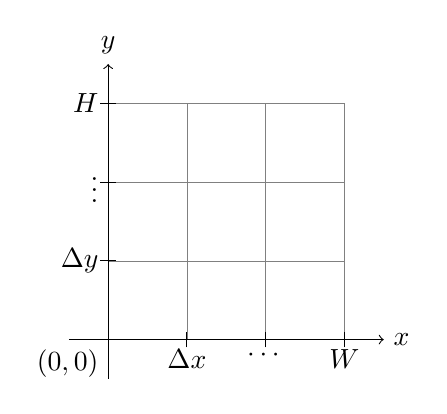
\begin{tikzpicture}
    
% Define the size of the cells
\def\Deltax{1} % Delta x size
\def\Deltay{1} % Delta y size
\def\Xmax{4} % Max X value
\def\Ymax{4} % Max Y value

% Draw the mesh
\foreach \x in {0,1,2} {
    \foreach \y in {0,1,2} {
        \draw[help lines] (\x*\Deltax,\y*\Deltay) grid (\x*\Deltax+\Deltax,\y*\Deltay+\Deltay);
    }
}

\node[below left] at (0,0) {$(0, 0)$};

% Draw axes
\draw[->] (-0.5,0) -- (3.5 *\Deltax,0) node[right] {$x$} ;
\draw[->] (0,-0.5) -- (0,3.5) node[above] {$y$};

% Add tick marks on x-axis with labels
\draw[shift={(1,0)}] (0,-0.1) -- (0,0.1);
\node[below] at (1, 0) {\(\Delta x\)};

\draw[shift={(2,0)}] (0,-0.1) -- (0,0.1);
\node[below] at (2, 0) {$\cdots$};

\draw[shift={(3,0)}] (0,-0.1) -- (0,0.1);
\node[below] at (3, 0) {$W$};

% Add tick marks on y-axis with labels

\draw[shift={(0,1)}] (-0.1,0) -- (0.1,0);
\node[left] at (0, 1) {$\Delta y$};
        
\draw[shift={(0,2)}] (-0.1,0) -- (0.1,0);
\node[left] at (0, 2) {$\vdots$};

\draw[shift={(0,3)}] (-0.1,0) -- (0.1,0);
\node[left] at (0, 3) {$H$};

\end{tikzpicture}
\caption{ Diskretizuota erdvė }
\end{figure}

\newpage
\subsection{Išreikštinis FTCS metodas}

Remiantis išreikštiniu FTCS (\textit{angl. forward time centered space}) metodu pakeisime sistemos \eqref{rect} lygtis su išvestinių aproksimacijomis gautomis skleidžiant išvestines pagal Teiloro eilutę.

\begin{subequations} \label{finite-diffs}
\begin{align}
	\frac{\partial c}{\partial t}\Big|_{x=x_i, y=y_j, t=t_n}
	&=\frac{c^{n+1}_{i,j}-c^n_{i,j}}{\Delta t} 
	+ \mathcal{O}(\Delta t)\\
	\frac{\partial^2c}{\partial x^2}\Big|_{x=x_i, y=y_j, t=t_n}
	&=\frac{c^n_{i-1,j} - 2c^n_{i,j} + c^n_{i+1,j}}{(\Delta x)^2} 
	+ \mathcal{O}((\Delta x)^2)\\
	\frac{\partial^2c}{\partial y^2}\Big|_{x=x_i, y=y_j, t=t_n}
	&=\frac{c^n_{i,j-1} - 2c^n_{i,j} + c^n_{i,j+1}}{(\Delta y)^2} 
	+ \mathcal{O}((\Delta y)^2)
\end{align}
\end{subequations}

Sudaryti skaitiniam modeliui naudosime standartinį žymėjimą baigtinių skirtumų operatoriams $\delta_x^2[c_{ij}]=c_{i-1,j}-2c_{i,j}+c_{i+1,j}$, $\delta_y^2[c_{ij}]=c_{i,j-1}-2c_{i,j}+c_{i,j+1}$. Įstatome aproksimacijas į matematinį modelį:

\begin{subequations} \label{numerical-eqs}
	\begin{align}
		\frac{c^{n+1}_{1,i,j}-c^n_{1,i,j}}{\Delta t} &=
		-3kc^{n}_{1,i,j}c^{n}_{2,i,j}
		+D_1\left(\frac{\delta_x^2[c^n_{1,i,j}]}{(\Delta x)^2}+\frac{\delta_y^2[c^n_{1,i,j}]}{(\Delta y)^2}\right) \\
		\frac{c^{n+1}_{2,i,j}-c^n_{2,i,j}}{\Delta t} &=
		-5kc^{n}_{1,i,j}c^{n}_{2,i,j}
		+D_2\left(\frac{\delta_x^2[c^n_{2,i,j}]}{(\Delta x)^2}+\frac{\delta_y^2[c^n_{2,i,j}]}{(\Delta y)^2}\right) \\
		\frac{c^{n+1}_{3,i,j}-c^n_{3,i,j}}{\Delta t} &=
		2kc^{n}_{1,i,j}c^{n}_{2,i,j}
		+D_3\left(\frac{\delta_x^2[c^n_{3,i,j}]}{(\Delta x)^2}+\frac{\delta_y^2[c^n_{3,i,j}]}{(\Delta y)^2}\right)
	\end{align}
\end{subequations}

Čia
$\Delta t$ - laiko žingsnis,
$\Delta x$ - diskrečios erdvės žingsnis $x$ ašimi,
$\Delta y$ - diskrečios erdvės žingsnis $y$ ašimi.
$c^n_{1,i,j}$, $c^n_{2,i,j}$, $c^n_{3,i,j}$ - atitinkamai pirmos, antros ir trečios medžiagų koncentracijos diskretizuotos erdvės tinklelio taške $(x_i, y_i, t_n)\in\omega$.
\newpage
\subsection{FTCS metodo skaitinis stabilumas}

Norint užtikrinti skaitinį programos stabilumą, reikia užtikrinti, kad visais laiko momentais, visuose diskretizuotos erdvės taškuose, visų medžiagų koncentracijos išliktų ne neigiamos. Šiai sąlygai išpildyti, užtenka pasirinkti pakankamai mažą laiko žingsnį $\Delta t$. Pirmiausia įvedame porą konstantų:
\begin{align*}
\mu_{mx} = \frac{D_m\Delta t}{(\Delta x)^2}, \quad
\mu_{my} = \frac{D_m\Delta t}{(\Delta y)^2}, \quad m = 1, 2, 3
\end{align*}
Tada pertvarkome dviejų dimensijų skaitinį modelį \eqref{numerical-eqs} taip, kad kairėse lygčių pusėse liktų medžiagų koncentracija laiko momentu $n+1$, o dešinėse lygčių pusėse sugrupuojame narius pagal medžiagų koncentraciją skirtinguose diskretizuotos erdvės taškuose:
\begin{subequations} \label{eqs:r-coefs}
  \begin{align}
  c^{n+1}_{1,i,j}&=
  \underbrace{(1-3k\Delta tc^{n}_{2,i,j}-2(\mu_{1x}+\mu_{1y}))}_{R_1}c^n_{1,i,j}
  +\mu_{1x}c^n_{1,i-1,j}+\mu_{1x}c^n_{1,i+1,j}+\mu_{1y}c^n_{1,i,j-1}+\mu_{1y}c^n_{1,i,j+1} \label{r-coefs1}\\
  c^{n+1}_{2,i,j}&=
  \underbrace{(1-5k\Delta tc^{n}_{1,i,j}-2(\mu_{2x}+\mu_{2y}))}_{R_2}c^n_{2,i,j}
  +\mu_{2x}c^n_{2,i-1,j}+\mu_{2x}c^n_{2,i+1,j}+\mu_{2y}c^n_{2,i,j-1}+\mu_{2y}c^n_{2,i,j+1} \label{r-coefs2}\\
  c^{n+1}_{3,i,j}&=
  \underbrace{(1-2(\mu_{3x} + \mu_{3y}))}_{R_3}c^n_{3,i,j}+2k\Delta tc^{n}_{1,i,j}c^{n}_{2,i,j} 
  +\mu_{3x}c^n_{3,i-1,j}+\mu_{3x}c^n_{3,i+1,j}
  +\mu_{3y}c^n_{3,i,j-1}+\mu_{3y}c^n_{3,i,j+1}
  \label{r-coefs3}
  \end{align}
\end{subequations}
Baziniu atveju, kai $n=0$, medžiagų koncentracija visuose taškuose yra ne neigiama, kaip numatyta pradinėse sąlygose \eqref{intial-cond}. Darome indukcijos hipotezės prielaidą, kad medžiagų koncentracija visuose diskretizuotos erdvės taškuose, laiko momentu $n$ bus ne neigiama:
\begin{align} \label{induction-assumption}
  c^n_{m,i,j} \geqslant 0, \quad m=1,2,3,\quad i=0,1,\dots,N-1,\quad j=0,1,\dots,M-1
\end{align}
% Akivaizdu, kad lygtyje \eqref{r-coefs3}, medžiagos koncentracija $c^{n+1}_{3,i,j}$ bus ne neigiama:
% \begin{align*}
%   \Delta t > 0 \land c^n_{m,i,j}\geqslant 0 \implies c^{n+1}_{3,i,j}=c^n_{3,i,j}+2\Delta tc^{n}_{1,i,j}c^{n}_{2,i,j}\geqslant 0 
% \end{align*}
Visose trijose medžiagų lygtyse, galima pastebėti, kad dėmenys su medžiagų koncentracijomis iš aplinkinių diskretizuotos erdvės taškų visada bus ne neigiami dėl prielaidos \eqref{induction-assumption} ir fakto, kad $\mu_{mx}>0$ ir $\mu_{my}>0$:
\begin{align*}
  \mu_{mx}c^n_{m,i-1,j}+\mu_{mx}c^n_{m,i+1,j}+\mu_{my}c^n_{m,i,j-1}+\mu_{my}c^n_{m,i,j+1}\geqslant 0 ,\quad m=1,2,3
\end{align*}
\newpage
Taigi, $c^{n+1}_{m,i,j}$ ženklą lemia tik koeficientai $R_1, R_2, R_3$, todėl įvedame ribojimą, kad $R_1\geqslant 0$, $R_2\geqslant 0$, $R_3\geqslant 0$. Turime nelygybių sistemą:
\begin{align} \label{impl-ineqs}
  \begin{cases}
    1-3k\Delta tc^{n}_{2,i,j}-2(\mu_{2x}+\mu_{2y})\geqslant 0\\
    1-5k\Delta tc^{n}_{1,i,j}-2(\mu_{1x}+\mu_{1y})\geqslant 0\\
    1-2(\mu_{3x}+\mu_{3y})\geqslant 0
  \end{cases}, \quad i=0,1,\dots,N-1, \quad j=0,1,\dots,M-1
\end{align}
Išreiškę nelygybes \eqref{impl-ineqs} per laiko žingsnį $\Delta t$ gauname:
\begin{align} \label{dt-ineq}
  \begin{cases}
    \Delta t \leqslant (3kc^{n}_{2,i,j}+2D_1((\Delta x)^{-2}+(\Delta y)^{-2}))^{-1}\\
    \Delta t \leqslant (5kc^{n}_{1,i,j}+2D_2((\Delta x)^{-2}+(\Delta y)^{-2}))^{-1}\\
    \Delta t \leqslant (2D_3((\Delta x)^{-2}+(\Delta y)^{-2})))^{-1}
  \end{cases}
\end{align}
% Gautas nelygybes galima apjungti dėl jų panašios struktūros. Norint, kad apjungta nelygybė tenkintų sistemą \eqref{dt-ineq}, reikia išrinkti mažiausią įmanomą laiko žingsnį $\Delta t$, o taip bus tada, kai trupmenos vardiklis bus kuo įmanoma didesnis. Dėl to gauta nelygybė įgaus formą:
% \begin{align}
%   \Delta t \leqslant \left(\max(3kc^{n}_{2,i,j}, 5kc^{n}_{1,i,j})+2D\left((\Delta x)^{-2}+(\Delta y)^{-2}\right)\right)^{-1}
% \end{align}

Turime tris nelygybes, kurios apibūdina laiko žingsnio $\Delta t$ apribojimus. Skaičiavimuose paprasčiausiai naudosime tą nelygybę, kuri apibūdina mažiausią laiko žingsinį. Parodėme, kad su pakankamai mažu laiko žingsniu $\Delta t$ išvengiame neigiamų sprendinio reikšmių. Tačiau čia sustoti būtų nenaudinga, nes turime rekursyvią priklausomybę -- norint pasirinkti $\Delta t$, reikia žinoti maksimalią medžiagų reikšmę simuliacijoje, o jai sužinoti reikia atlikti simuliaciją su pasirinktu laiko žingsniu $\Delta t$.

Parodysime, kad galima panaikinti laiko žingsnio priklausomybę nuo laiko momento $n$ ir kad $\Delta t$ priklauso tik nuo pradinių sąlygų $c^0_{1,i,j}$ ir $c^0_{2,i,j}$. Medžiagos kiekį sistemoje galima gauti integravus medžiagos koncentraciją erdvėje:

\begin{align}
  q&=\int_\Omega c dV \label{quantity-general}
\end{align}

Iš čia galime išvesti išraišką medžiagos kiekio pokyčiui per laiką:

\begin{align}
  \frac{\partial q}{\partial t}=\frac{\partial}{\partial t}\int_\Omega c dV=\int_\Omega\frac{\partial c}{\partial t}dV,
\end{align}

Įstatome pirmų dviejų medžiagų lygtis iš matematinio modelio \eqref{rect} ir gauname lygtis pirmos $q_1$ ir antros $q_2$ medžiagos kiekio pokyčiams per laiką:
\begin{align}
  \frac{\partial q_1}{\partial t}
  =-3k\int_\Omega c_1c_2\,dV 
  + D_1\int_\Omega \Delta c_1\,dV
  =-3k\int_\Omega c_1c_2\,dV 
  + D_1\int_\Omega \nabla \cdot (\nabla c_1)\,dV\\
  \frac{\partial q_2}{\partial t}
  =-5k\int_\Omega c_1c_2\,dV 
  + D_2\int_\Omega \Delta c_2\,dV
  =-5k\int_\Omega c_1c_2\,dV 
  + D_2\int_\Omega \nabla \cdot (\nabla c_2)\,dV
\end{align}
\newpage
Pagal Gauso-Ostrogradskio divergencijos teoremą ir kraštinę sąlygą \eqref{general-boundary-cond} gauname, kad:
\begin{align}\label{no-q-change}
\int_\Omega \nabla \cdot (\nabla c_m) dV = \int_{\partial\Omega} \nabla c_m \cdot \vec{n}\, dS = 0,\quad m=1,2
\end{align}
Todėl pirmos ir antros medžiagų kiekio pokytis per laiką bus ne teigiamas:
\begin{subequations} \label{negative-quantity}
\begin{align}
  \frac{\partial q_1}{\partial t}=-3k\int_\Omega c_1c_2\,dV \leqslant 0\\
  \frac{\partial q_2}{\partial t}=-5k\int_\Omega c_1c_2\,dV\leqslant 0
\end{align}
\end{subequations}
Tai reiškia, kad maksimalios pirmos ir antros medžiagų reikšmės bus laiko momente $n=0$, tad nelygybę galime suprastinti iki šios formos:
\begin{align}
  \begin{cases}
    \Delta t \leqslant (3kc^{0}_{2,i,j}+2D_1((\Delta x)^{-2}+(\Delta y)^{-2}))^{-1}\\
    \Delta t \leqslant (5kc^{0}_{1,i,j}+2D_2((\Delta x)^{-2}+(\Delta y)^{-2}))^{-1}\\
    \Delta t \leqslant (2D_3((\Delta x)^{-2}+(\Delta y)^{-2})))^{-1}
  \end{cases}
\end{align}
Laiko žingsnis čia vis dar priklauso nuo diskretizuotos erdvės koordinatės $(x_i, y_j)$, tačiau nesunku pastebėti, kad užtenka parinkti didžiausią reikšmę iš kiekvienos pradinės sąlygos -- tokiu būdu laiko žingsnis gausis mažiausias. Iš pradinės sąlygos \eqref{intial-cond} turime:
\begin{align*}
\max c^0_{1,i,j}=3c_0,\quad i=0,1,\dots,N-1, \quad j=0,1,\dots,M-1\\
\max c^0_{2,i,j}=5c_0,\quad i=0,1,\dots,N-1, \quad j=0,1,\dots,M-1
\end{align*}
Taigi, kad simuliacija išliktų skaitiškai stabili, reikia, kad laiko žingsnis $\Delta t$ tenkintų šią nelygybę.
\begin{align} \label{numerical-stability-condition}
  \begin{cases}
    \Delta t \leqslant (15kc_0+2D_1((\Delta x)^{-2}+(\Delta y)^{-2}))^{-1}\\
    \Delta t \leqslant (15kc_0+2D_2((\Delta x)^{-2}+(\Delta y)^{-2}))^{-1}\\
    \Delta t \leqslant (2D_3((\Delta x)^{-2}+(\Delta y)^{-2})))^{-1}
  \end{cases}
\end{align}


\newpage
\subsection{Neišreikštinis kintamos krypties metodas}

Neišreikštinį kintamos krypties metodą (\textit{alternating direction implicit, ADI}) JAV mokslininkai Donald W. Peaceman ir Henry H. Rachford Jr. pristatė savo straipsnyje \enquote{Skaitinis sprendinys parabolinėms ir elipsinės diferencialinėms lygtims} \cite{doi:10.1137/0103003}. Nuo to laiko šis metodas plačiai taikomas matematinio modeliavimo srityje. Kaip galima suprasti iš straipsnio pavadinimo, šis metodas pritaikytas spręsti parabolines ir elipsines diferencialinių lygčių sistemas. Kadangi mūsų nagrinėjamą sistemą sudaro parabolinės diferencialinės lygtys, jį ir taikysime.

Šis metodas yra tarpinis variantas tarp išreikštinio FTCS ir Crank-Nicholson metodo, kuriuo bandoma išlaikyti sprendimo greitį ir tikslumą. Įprastoms parabolinėms lygtims šis metodas būna besąlygiškai stabilus \cite{liAlternatingDirectionImplicit2021}, tai leidžia pasirinkti bet kokio dydžio laiko žingsnį ir tokiu būdu sumažinti bendrą laiko žingsnių kiekį, kurį reikia įvykdyti. Toliau pritaikysime metodą nagrinėjamai sistemai.

Užuot tiesiogiai skaičiavę skaitinį sprendinį sekančiu laiko momentu $c^{n+1}_{m,i,j}$, pirmiausia apskaičiuosime tarpinį sprendinį, kurį žymėsime $c^*_{m,i,j}$. Skaitiniam modeliui sudaryti naudosime tas pačias išvestinių aproksimacijas, kurias naudojome FTCS metode, tačiau pagal ADI metodo specifiką laikysime, kad difuzijos komponenta sudaro išreikštinė ir neišreikštinė dalys -- \hbox{t. y.} $x$ ašies išvestinei skaičiuoti bus naudojamas ateinančio laiko žingsnio sprendinys $c^*$, o $y$ ašies išvestinei naudosime jau turimą sprendinį $c^n$. Dėl priežasčių, kurios bus atskleistos vėliau, reakcijos komponentus visada skaičiuosime pagal jau turimą laiko žingsnį $c^n$. Sudarome lygtis tarpiniam sprendiniui $c^*$ pasinaudojant standartiniu baigtinių skirtumų operatorių žymėjimu, kurį naudojome ir FTCS modeliui $\delta_x^2[c_{ij}]=c_{i-1,j}-2c_{i,j}+c_{i+1,j}$, $\delta_y^2[c_{ij}]=c_{i,j-1}-2c_{i,j}+c_{i,j+1}$:
\begin{subequations} \label{eqs:adi-half-step}
\begin{align}
	\frac{c^*_{1,i,j} - c^n_{1,i,j}}{\frac{1}{2}\Delta t} &= D_1 \left( \frac{\delta_x^2[c^*_{1,i,j}]}{(\Delta x)^2} + \frac{\delta_y^2[c^n_{1,i,j}]}{(\Delta y)^2} \right) - 3kc^n_{1,i,j}c^n_{2,i,j}\\
	\frac{c^*_{2,i,j} - c^n_{2,i,j}}{\frac{1}{2}\Delta t} &= D_2 \left( \frac{\delta_x^2[c^*_{2,i,j}]}{(\Delta x)^2} + \frac{\delta_y^2[c^n_{2,i,j}]}{(\Delta y)^2} \right) - 5kc^n_{1,i,j}c^n_{2,i,j}\\
	\frac{c^*_{3,i,j} - c^n_{3,i,j}}{\frac{1}{2}\Delta t} &= D_3 \left( \frac{\delta_x^2[c^*_{3,i,j}]}{(\Delta x)^2} + \frac{\delta_y^2[c^n_{3,i,j}]}{(\Delta y)^2} \right) +2kc^n_{1,i,j}c^n_{2,i,j}
\end{align}
\end{subequations}

Analogiškas lygtis yra sudaromos sprendiniui $c^{n+1}$ rasti, tačiau apkeičiame sprendinius, kuriuos naudojame difuzijos komponentui -- $x$ ašies išvestinei naudosime jau turimą sprendinį $c^{*}$, o $y$ ašies naudosime sekančio laiko žingsnio sprendinį $c^{n+1}$:

\begin{subequations} \label{eqs:adi-next-step}
\begin{align}
	\frac{c^{n+1}_{1,i,j} - c^*_{1,i,j}}{\frac{1}{2}\Delta t} 
	&= D_1 \left( \frac{\delta_x^2[c^{*}_{1,i,j}]}{(\Delta x)^2} 
	+ \frac{\delta_y^2[c^{n+1}_{1,i,j}]}{(\Delta y)^2} \right) - 3kc^*_{1,i,j}c^*_{2,i,j}\\
	\frac{c^{n+1}_{2,i,j} - c^*_{2,i,j}}{\frac{1}{2}\Delta t} 
	&= D_2 \left( \frac{\delta_x^2[c^*_{2,i,j}]}{(\Delta x)^2}
	+ \frac{\delta_y^2[c^{n+1}_{2,i,j}]}{(\Delta y)^2} \right) - 5kc^*_{1,i,j}c^*_{2,i,j}\\
	\frac{c^{n+1}_{3,i,j} - c^*_{3,i,j}}{\frac{1}{2}\Delta t} 
	&= D_3 \left( \frac{\delta_x^2[c^*_{3,i,j}]}{(\Delta x)^2} 
	+ \frac{\delta_y^2[c^{n+1}_{3,i,j}]}{(\Delta y)^2} \right) +2kc^*_{1,i,j}c^*_{2,i,j}
\end{align}
\end{subequations}

\newpage

Kitaip nei FTCS metodo atveju, sprendinys, kurį bandome rasti, priklauso ne tik nuo praėjusio laiko žingsnio sprendinio, bet ir nuo paties savęs. Tai galioja tiek tarpiniam, tiek sekančio žingsnio sprendiniui. Rezultate mes gauname lygčių sistemą, kurią reikia spręsti. Iš pradžių persitvarkysime gautas lygtis tarpiniam sprendiniui $c^*$, susikeldami skirtingų laiko žingsnių sprendinių komponentus į skirtingas lygybės puses. Kadangi lygtis yra labai panašios viena į kitą jas pertvarkysime bendrai žymėdami medžiagos indeksą $m$, reakcijos koeficientus $\alpha_1 = -3$, $\alpha_2 = -5$, $\alpha_3 = 2$. Taip pat naudosime žymėjimą konstantoms: $\mu_{mx} = \frac{\Delta t D_m}{2(\Delta x)^2}$, $\mu_{my} = \frac{\Delta t D_m}{2(\Delta y)^2}$, $\mu_m = \frac{1}{2} \Delta t \alpha_m k$.

\begin{align*}
  \frac{c^{*}_{m,i,j} - c^n_{m,i,j}}{\frac{1}{2}\Delta t} 
  &= D_m \left( \frac{\delta_x^2[c^{*}_{m,i,j}]}{(\Delta x)^2} 
  + \frac{\delta_y^2[c^n_{m,i,j}]}{(\Delta y)^2} \right) 
  + \alpha_mkc^*_{1,i,j}c^*_{2,i,j} \\
  c^*_{m,i,j} 
  &= \frac{1}{2}\Delta t D_m \left( \frac{\delta_x^2[c^{*}_{m,i,j}]}{(\Delta x)^2} 
  + \frac{\delta_y^2[c^n_{m,i,j}]}{(\Delta y)^2} \right)
  + \frac{1}{2}\Delta t \alpha_m kc^n_{1,i,j}c^n_{2,i,j} + c^n_{m,i,j}\\
  c^*_{m,i,j} - \underbrace{\frac{\Delta t D_m}{2(\Delta x)^2}}_{\mu_{mx}}\delta_x^2[c^{*}_{m,i,j}] 
  &= \underbrace{\frac{\Delta t D_m}{2(\Delta y)^2}}_{\mu_{my}}\delta_y^2[c^n_{m,i,j}]
  + \underbrace{\frac{1}{2}\Delta t \alpha_m k}_{\mu_m}c^n_{1,i,j}c^n_{2,i,j} + c^n_{m,i,j}\\
  c^*_{m,i,j} - \mu_{mx}\delta_x^2[c^{*}_{m,i,j}]
  &= \mu_{my}\delta_y^2[c^n_{m,i,j}] + \mu_m c^n_{1,i,j}c^n_{2,i,j} + c^n_{m,i,j}
\end{align*}

Išskleidę paskutinė lygtyje esančius baigtinių skirtumų operatorius gauname lygtį tarpiniam sprendiniui $c^*$:

\begin{align}
  -\mu_{mx}c^{*}_{m,i-1,j}+(1+2\mu_{mx})c^{*}_{m,i,j}-\mu_{mx}c^{*}_{m,i+1,j}
  &= \mu_{my}c^n_{m,i,j-1}+(1-2\mu_{my})c^n_{m,i,j}+\mu_{my}c^n_{m,i,j+1}+\mu_m c^n_{1,i,j}c^n_{2,i,j}
\end{align}

Analogiškai galima išvesti lygtis sekančiam laiko žingsniui $c^{n+1}_{m,i,j}$:

\begin{align}
  % c^{n+1}_{m,i,j} - \mu_{my}\delta_y^2[c^{n+1}_{m,i,j}]
  % &= \mu_{mx}\delta_x^2[c^*_{m,i,j}] + \mu_m c^*_{1,i,j}c^*_{2,i,j} + c^*_{m,i,j}\\
  -\mu_{my}c^{n+1}_{m,i,j-1}+(1+2\mu_{my})c^{n+1}_{m,i,j}-\mu_{my}c^{n+1}_{m,i,j+1}
  &= \mu_{mx}c^*_{m,i-1,j}+(1-2\mu_{mx})c^*_{m,i,j}+\mu_{mx}c^*_{m,i+1,j}+\mu_m c^*_{1,i,j}c^*_{2,i,j}
\end{align}

Kraštinėms sąlygoms apskaičiuoti naudosime centrinę pirmosios išvestinės aproksimaciją:

\begin{align*}
  \frac{\partial c}{\partial x}\Big|_{x=x_i, y=y_j, t=t_n} 
  &\approx \frac{c^n_{i+1,j}-c^n_{i-1,j}}{2\Delta x} &
  \frac{\partial c}{\partial y}\Big|_{x=x_i, y=y_j, t=t_n} 
  &\approx \frac{c^n_{i,j+1}-c^n_{i,j-1}}{2\Delta y}
\end{align*}

Įstate šias aproksimacijas į modelio kraštines sąlygas \eqref{boundary-cond} gauname:

\begin{subequations} \label{boundary-cond-approx}
\begin{align} 
  c_{i+1,j} &= c_{i-1,j}, \text{ kai } i = 0 \text{ arba } i = N-1 &
  c_{i,j+1} &= c_{i,j-1}, \text{ kai } j = 0 \text{ arba } j = M-1 &
\end{align}
\end{subequations}

Turint kraštines sąlygas \eqref{boundary-cond-approx} bei lygtis \eqref{eqs:adi-half-step} ir \eqref{eqs:adi-next-step} galime užrašyti sistemas matricos pavidalu. Pirmiausia užrašome lygčių sistemas tarpiniam sprendiniui $c^*$:

\begin{align*}
  \resizebox{\textwidth}{!}{$
  \begin{bmatrix}
    1 + 2\mu_{mx} & -2\mu_{mx} & 0 & \cdots & 0 & 0\\
    -\mu_{mx} & 1 + 2\mu_{mx} & -\mu_{mx} & \cdots & 0 & 0\\
    0 & -\mu_{mx} & 1 + 2\mu_{mx} & \cdots & 0 & 0\\
    \vdots & \vdots & \vdots & \ddots & \vdots & \vdots\\
    0 & 0 & 0 & \cdots & 1 + 2\mu_{mx} & -\mu_{mx}\\
    0 & 0 & 0 & \cdots & -2\mu_{mx} & 1 + 2\mu_{mx}
  \end{bmatrix}
  \begin{bmatrix}
    c^*_{m,0,j}\\
    c^*_{m,1,j}\\
    c^*_{m,2,j}\\
    \vdots\\
    c^*_{m,N-1,j}
  \end{bmatrix}
  =
  \begin{bmatrix}
    \mu_{my}c^n_{m,0,j-1}+(1-2\mu_{my})c^n_{m,0,j}+\mu_{my}c^n_{m,0,j+1}+\mu_m c^n_{1,0,j}c^n_{2,0,j}\\
    \mu_{my}c^n_{m,1,j-1}+(1-2\mu_{my})c^n_{m,1,j}+\mu_{my}c^n_{m,1,j+1}+\mu_m c^n_{1,1,j}c^n_{2,1,j}\\
    \mu_{my}c^n_{m,2,j-1}+(1-2\mu_{my})c^n_{m,2,j}+\mu_{my}c^n_{m,2,j+1}+\mu_m c^n_{1,2,j}c^n_{2,2,j}\\
    \vdots\\
    \mu_{my}c^n_{m,N-1,j-1}+(1-2\mu_{my})c^n_{m,N-1,j}+\mu_{my}c^n_{m,N-1,j+1}+\mu_m c^n_{1,N-1,j}c^n_{2,N-1,j}
  \end{bmatrix}
  $}
\end{align*}

Lygčių sistemos sekančio laiko žingsnio sprendiniui $c^{n+1}$:

\begin{align*}
  \resizebox{\textwidth}{!}{$
  \begin{bmatrix}
    1 + 2\mu_{my} & -2\mu_{my} & 0 & \cdots & 0 & 0\\
    -\mu_{my} & 1 + 2\mu_{my} & -\mu_{my} & \cdots & 0 & 0\\
    0 & -\mu_{my} & 1 + 2\mu_{my} & \cdots & 0 & 0\\
    \vdots & \vdots & \vdots & \ddots & \vdots & \vdots\\
    0 & 0 & 0 & \cdots & 1 + 2\mu_{my} & -\mu_{my}\\
    0 & 0 & 0 & \cdots & -2\mu_{my} & 1 + 2\mu_{my}
  \end{bmatrix}
  \begin{bmatrix}
    c^*_{m,i,0}\\
    c^*_{m,i,1}\\
    c^*_{m,i,2}\\
    \vdots\\
    c^*_{m,i,M-1}
  \end{bmatrix}
  =
  \begin{bmatrix}
    \mu_{mx}c^n_{m,i-1,0}+(1-2\mu_{mx})c^n_{m,i,0}+\mu_{mx}c^n_{m,i+1,0}+\mu_m c^n_{1,i,0}c^n_{2,i,0}\\
    \mu_{mx}c^n_{m,i-1,1}+(1-2\mu_{mx})c^n_{m,i,1}+\mu_{mx}c^n_{m,i+1,1}+\mu_m c^n_{1,i,1}c^n_{2,i,1}\\
    \mu_{mx}c^n_{m,i-1,2}+(1-2\mu_{mx})c^n_{m,i,2}+\mu_{mx}c^n_{m,i+1,2}+\mu_m c^n_{1,i,2}c^n_{2,i,2}\\
    \vdots\\
    \mu_{mx}c^n_{m,i-1,M-1}+(1-2\mu_{mx})c^n_{m,i,M-1}+\mu_{mx}c^n_{m,i+1,M-1}+\mu_m c^n_{1,i,M-1}c^n_{2,i,M-1}
  \end{bmatrix}
  $}
\end{align*}

Šios sistemos sprendinys yra atitinkamai ieškomo laiko žingsnio sprendinio eilutė arba stulpelis, todėl kiekvieno laiko žingsnio sprendiniui rasti šią sistemą reikės spręsti $M + N$ kartų. Taip pat galima pastebėti, kad kairėje lygties pusėje esančios matricos yra tridiagonalinės, todėl jas galima spręsti efektyviai naudojant tridiagonalinės matricos algoritmą. Būtent dėl šios priežasties mes pasirinkome laikyti reakcijos komponentus išreikštinais, kitu atveju matricos nebūtų tridiagonalinės. Šis sprendimas turi ir savo minusų -- kadangi reakcijos dėmuo laikomas išreikštiniu, sistema nebėra besąlygiškai stabili.
\section{Skaitinių modelių įgyvendinimas ir jų rezultatai}

Skaitiniams modeliams įgyvendinti buvo pasirinkta \textit{Python} programavimo kalba. \textit{Python} turi didelį kiekį bibliotekų, skirtų skaitiniams skaičiavimams, tokių kaip \textit{NumPy}, \textit{SciPy}, \textit{Matplotlib}, kurios leidžia efektyviai dirbti su dideliais duomenų rinkiniais ir atlikti sudėtingus skaičiavimus.

Modelio rezultatai yra saugomi kaip atskiri \textit{.npy} formato failai, kurie yra skirti saugoti \mbox{\textit{NumPy}} masyvus. Dėl praktinių rezultatų panaudojimo ir tyrimo nebūtina saugoti informacijos apie visus laiko žingsnius, todėl išsaugotuose rezultatų failuose, simuliacijos kadrai laiko kryptimi gali būti praretinti iki tūkstančio kartų, priklausomai nuo pasirinktų parametrų. Pagalbiniai duomenų vaizdavimo skriptai šiuos duomenis agreguoja į grafikus, kurie išsaugomi \textit{.png} formatu.

Norint praktiškai panaudoti ADI metodą, būtina užtikrinti, kad tridiagonalinės sistemos būtų sprendžiamos efektyviai, tam buvo naudojama \textit{SciPy} funkcija \texttt{solve\_banded}

\subsection*{Medžiagos kiekis}

Dėl didelės rezultatų dimensijos būtų sunku interpretuoti grafiškai pavaizduotus sprendinio duomenis, todėl tyrimui yra naudinga vizualizuoti ir medžiagų kiekius sistemoje. Galime išskleisti formulę medžiagos kiekiui bendru atveju \eqref{quantity-general} ir gausime formulę diskrečiam atvejui \cite{strangCalculusVolume32016}:
\begin{align}
    q(t) = \int_\Omega c\,dV = \int_0^W \int_0^H c(x, y, t)\,dy\,dx
\end{align}
Pakeičiam dvigubą integralą su dviguba Rymano suma ir gaunam, kad medžiagos $c_m$ kiekis diskrečiu laiko momentu $n$ yra:
\begin{align}
    q_{m, n}= \sum_{i=0}^{N-1}\sum_{j=0}^{M-1} c_{m, i,j}^n \frac{W\cdot H}{N\cdot M} \quad m=1, 2, 3
\end{align}

Toliau nagrinėdami kompiuterinio modelio rezultatus naudosime šį žymėjimą. Šis indikatorius žymi kaip tam tikros medžiagos kiekis sistemoje keičiasi einant laikui, pavyzdžiui - pirma ir antra medžiagos reaguoja ir sukuria trečią medžiagą todėl turėtume matyti, kad pirmos ir antros medžiagos kiekiai per laiką mažėja, o trečios medžiagos kiekis per laiką auga.

\newpage
\subsection{Modelių rezultatai}

\subsubsection{Išreikštinis FTCS metodas}

\begin{figure}[h!]
\centering
\includegraphics[width=0.75\textwidth]{images/example-0.png} \\ 
\includegraphics[width=0.75\textwidth]{images/example-1.png} \\
\includegraphics[width=0.75\textwidth]{images/example-2.png}

\caption{Kompiuterinio modelio rezultato pavyzdys su parametrais gautais eksperimentiniu būdu, kai reakcija vyksta temperatūroje $T=1600\degree C$ \cite{mackeviciusCloserLookComputer2012}. Parametrų reikšmės: $D = 28\times 10^{-6} \frac{\mu m^2}{s}$, $W = \sqrt[3]{10}\mu m$, $H = \sqrt[3]{10}\mu m$, $\Delta x = \frac{\sqrt[3]{10}}{79}\mu m$, $\Delta y = \frac{\sqrt[3]{10}}{79} \mu m$, $k = 192 \frac{1}{ \frac{g}{\mu m^3}\cdot s}$, $c_0 = 10^{-6} \frac{g}{\mu m^3}$, $\Delta t \approx 6.5157s$ - pasirinktas pagal \eqref{numerical-stability-condition} }

\label{result-example}
\end{figure}

\ref{result-example}-ame pavyzdys vaizduoja kompiuterinio (YAG) reakcijos modelio rezultatus, kurie yra išdėstyti vertikaliai kiekvienai medžiagai $c_1, c_2, c_3$. Kiekvienas kadrų stulpelis vaizduoja visų medžiagų koncentracijas tuo pačiu laiko momentu. Pavyzdyje nurodyti parametrai bus naudojami tolesniems pavyzdžiams ir nebus išreikštinai dar kartą nurodomi nebent jie keičiasi. Taip pat kai kuriose vietose praleisime antros medžiagos $c_2$ vaizdavimą, nes jos koncentracijos pasiskirstymas yra simetriškas pirmos medžiagos $c_1$ pasiskirstymui.

\newpage

\begin{figure}[h!]
\centering
\includegraphics[width=\textwidth]{images/T1200-c0-1.png} \\ 
% \includegraphics[width=\textwidth]{images/T1200-c1-1.png}  \\
\includegraphics[width=\textwidth]{images/T1200-c2-1.png} 

\caption{Kompiuterinio modelio rezultato pavyzdys su parametrais gautais eksperimentiniu būdu, kai reakcija vyksta temperatūroje $T=1200\degree C$ \cite{mackeviciusCloserLookComputer2012}. Parametrų reikšmės: $D = 10.5\times 10^{-6} \frac{\mu m^2}{s}$, $k = 119 \frac{1}{ \frac{g}{\mu m^3}\cdot s}$, $\Delta t \approx 17.1651s$ - pasirinktas pagal \eqref{numerical-stability-condition} }

\label{alternate-result-example}
\end{figure}

\ref{alternate-result-example}-ame pavyzdyje matome kaip atrodo modelio rezultatai, kai parinkti parametrai atitinka reakcijos sąlygas, kuri vyksta prie temperatūros $T=1200\degree$. Šie rezultatai atitinka praktikoje pastebimą faktą, kad ši reakcija prie aukštesnės temperatūros vyksta greičiau \cite{ivanauskasComputationalModellingYAG2009}. 

\subsubsection{ADI metodas}

\begin{figure}[h!]
  \centering
  \includegraphics[width=0.75\textwidth]{images/adi/c1-1000C.png} \\ 
  \includegraphics[width=0.75\textwidth]{images/adi/c3-1000C.png}
  
  \caption{ADI modelio rezultatas, kai reakcijos temperatūra $T=1000\degree C$ (parametrai tokie patys kaip \ref{result-example}-ame pavyzdyje.}
  
  \label{fig:adi-result-T-1000}
\end{figure}

\begin{figure}[h!]
    \centering
    \includegraphics[width=0.75\textwidth]{images/adi/c1-1600C.png} \\ 
    \includegraphics[width=0.75\textwidth]{images/adi/c3-1600C.png}
    
    \caption{ADI modelio rezultatas, kai reakcijos temperatūra $T=1600\degree C$ (parametrai tokie patys kaip \ref{result-example}-ame pavyzdyje.}
    
    \label{fig:adi-result-T-1600}
  \end{figure}

\subsection{Programos korektiškumo tikrinimas}

\subsubsection*{Korektiškumo tikrinimas bendru atveju}

Nagrinėjant programos korektiškumą naudosime modelio rezultatų duomenis. 
Norint nustatyti, ar programa veikia korektiškai galima tikrinti, ar mažinant žingsnių dydį, skaitinis sprendinys artėja prie tikrojo sprendinio. Šiuo atveju mažinsime erdvės žingsnius $\Delta x$ ir $\Delta y$. Tai lemia diskretaus tinklelio taškų kiekio padidėjimą, nes egzistuoja atvirkštinė priklausomybė tarp erdvinių žingsnių dydžio ir diskrečių taškų kiekio atitinkamomis ašimis (\ref{meshx}, \ref{meshy}).

\newpage

\begin{figure}[h!]
    \centering
    \includegraphics[width=\textwidth]{images/space-error-1.png}

    \caption{Kompiuterinio modelio rezultatai - sprendinio tikslumo priklausomybė nuo diskrečių taškų skaičiaus. }

    \label{results-space-error}
\end{figure}

\ref{results-space-error}-ame pav. matome, kad eksponentiškai didinant diskrečių taškų skaičių, sprendinių grafikai tolygiai artėja prie sprendinio su didžiausiu tikslumu, darome prielaidą, kad didinant diskrečių taškų skaičių, skaitinis sprendinys konverguoją į tikrąjį sprendinį. Kažkuriuo momentu diskrečios erdvės taškų kiekio didinimas nebeduoda ypatingai didelių rezultato pagerėjimų. Sprendinių grafikuose taip pat galima įžvelgti, kad pirmų dviejų medžiagų kiekiai per laiką griežtai ne mažėja - tai mes teoriškai parodėme \eqref{negative-quantity}, taip, žinoma, yra dėl  medžiagų reakcijos. 

Analogiškai galima būtų fiksuoti erdvinius žingsnius $\Delta x, \Delta y$ ir stebėti kaip keičiasi skaitinis sprendinys mažinant laiko žingsnį $\Delta t$. Dėl priežasčių, kurios vėliau bus akivaizdžios vaizduosime du sprendinius - vienas iš jų gautas pasirinkus $\Delta t$ pagal \eqref{numerical-stability-condition}, o kitam paimta konkreti reikšmė $\Delta t = 10^{-4}$.


\begin{figure}[h!]

\centering

\includegraphics[width=\textwidth]{images/time-error-1.png}

\caption{Kompiuterinio modelio rezultatai - sprendinio priklausomybė nuo laiko žingsio pasirinkimo. Čia reakcijos laikas $T=16h$.}

\label{time-error}

\end{figure}

\ref{time-error}-ame pav. matome, kad sprendiniai yra identiški. Laiko žingsnio  $\Delta t$ pasirinkimas pagal \eqref{numerical-stability-condition} yra pakankamai geras ir mažesnių laiko žingsnių pasirinkimas neduoda pastebimai tikslesnių rezultatų.

\newpage
\subsubsection*{Korektiškumo tikrinimas kai vyksta tik difuzija}

Jei reakcijos koeficientas būtų lygus nuliui, vienintelis sistemoje vykstantis procesas būtų pirmų dviejų medžiagų difuzija. Jei skaitinis modelis veikia korektiškai, rezultatuose turėtų būti galima matyti, kad difuzijos metu medžiagos kiekis sistemoje nekinta, tai teoriškai parodėme skyriuje apie skaitinį stabilumą \eqref{no-q-change}.

\begin{figure}[h!]
    \centering
    \includegraphics[width=0.5\textwidth]{images/only-diff-1.png}
    \caption{Kompiuterinio modelio rezultatai - medžiagų kiekių priklausomybė nuo laiko, kai reakcija nevyksta. Čia diskrečių laiko žingsnių skaičius $\tau=10^4$, o reakcijos greitis $k = 0$. }
    \label{no-reaction}
\end{figure}

\ref{no-reaction}-ame pavyzdyje kompiuterinės programos rezultatai yra būtent tokie, kokių tikėjomės, tačiau iš šio grafiko negalime užtikrinti, kad simuliacijoje išvis kažkas vyksta. Norint patikrinti, ar medžiagos difunduoja korektiškai galime pabandyti pavaizduoti medžiagų kiekį visoje srityje $\Omega$ kaip rezultatų pavyzdyje \eqref{result-example}.

\begin{figure}[h!]
\centering
\includegraphics[width=\textwidth]{images/all-only-diff-1.png} \\
\includegraphics[width=\textwidth]{images/all-only-diff-2.png}

\caption{Kompiuterinio modelio rezultatai - medžiagų koncentracijų pasiskirstymas per laiką, kai vyksta tik difuzija. Čia diskrečių laiko žingsnių skaičius $\tau=10^4$, o reakcijos greitis $k = 0$. }

\label{only-diffusion}
\end{figure}

\ref{only-diffusion}-ame pavyzdyje akivaizdžiai matosi, kad medžiagų difuzija vyksta įprastai. Einant laikui, medžiagos iš didesnės koncentracijos sričių juda į sritis, kur koncentracija yra mažesnė. Reakcijai einant į pabaigą matome, kad medžiagos tolygiai pasiskirsto po erdvę.




\section{Maišymo modeliavimas}

\subsection{Atsitiktinis maišymas}

Konstruojant kompiuterinį modelį šiam procesui atkreipsime dėmesį į kelias svarbias detales:

\begin{itemize}
  \item Išmaišymas vyksta prie daug žemesnės temperatūros negu reakcija
  \item Išmaišymas gali vykti kelis kartus
  \item Išmaišymo procesas nėra deterministinis
\end{itemize}

\subsubsection*{Maišymas prie žemesnės temperatūros}

Kadangi maišymas vyksta prie daug žemesnės temperatūros negu pati reakcija, darysime prielaidą, kad ištraukus reagentus iš krosnies cheminė reakcija ir difuzija nevyksta, todėl medžiagų maišymą modeliuosime kaip momentinį procesą, kuris įvyksta tarp diskrečių laiko žingsnių.

\subsubsection*{Maišymas kelis kartus}

Praktikoje vykdant šią reakcija chemikai savo nuožiūra pasirenka laiką, kuriuo vykdys išmaišymą, todėl ir kompiuterinis modelis turėtų suteikti vartotojui pasirinkimą nurodyti konkrečius laiko momentus, kada vyks medžiagų išmaišymas. Šiuos laikus žymėsime taip:

\begin{align}
    t^1_\text{mix}, t^2_\text{mix}, \dots, t^{T^*}_\text{mix} \quad T^*\in \mathbb{N}
\end{align}

Čia $T^*$ -- bendras išmaišymų skaičius, o $t^i_\text{mix}$ -- $i$-tojo išmaišymo laikas. Kadangi kompiuterinis modelis laiko informaciją apie diskrečius laiko taškus $t_n$, mes negalime tiesiogiai apibrėžti sąlygos, kad išmaišymas vyks konkrečiu laiko momentu $t^i_\text{mix}$, todėl medžiagas išmaišysime einamajame laiko žingsnyje $t_n$, kuris yra artimiausias išmaišymo laikui $t^i_\text{mix}$:

\begin{figure}[!h]
\centering
\label{mix-inequality-graphic}
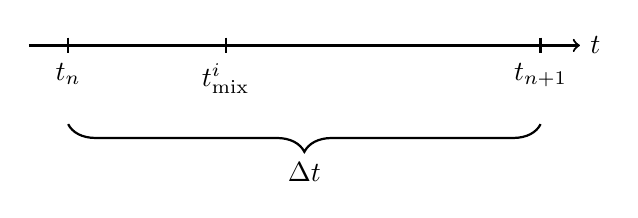
\begin{tikzpicture}[thick]

% Main timeline
\draw[->] (-0.5,0) -- (6.5,0) node[right] {$t$}; % Timeline with axis label

% Time points
\foreach \x/\label in {0/{$t_n$}, 2/{$t^i_\text{mix}$}, 6/{$t_{n+1}$}} {
    \draw (\x,0.1) -- (\x,-0.1) node[below] {\label};
}

% Braces for interval
\draw[decorate,decoration={brace,amplitude=10pt,mirror}] (0,-1) -- (6,-1) node[midway,below=10pt] {$\Delta t$};


\end{tikzpicture}
\caption{Šiuo atveju, išmaišymas įvyks laiko žingsniu $t_n$, o ne $t_{n+1}$, nes $t^i_\text{mix}$ yra arčiau laiko momento $t_n$}
\end{figure}

arba kitaip sakant išmaišymas įvyks laiko žingsniu $t_n$, jei:

\begin{align}
    \vert t_n - t^i_\text{mix} \vert < \frac{1}{2}\Delta t \label{mix-inequality}
\end{align}

\newpage

\subsubsection*{Atsitiktinis maišymas}

Maišymas praktikoje yra chaotiškas procesas, todėl sudarydami kompiuterinį modelį turime į tai atsižvelgti. Maišymą modeliuosime kaip reakcijos erdvės sričių atsitiktinį išdėstymą. Pradinė sritį $\Omega$ padalinsime į mažesnes, nepersidengiančias, vienodas kvadratines sritis $\Omega_i$, tada sugeneruosime atsitiktinę $4$-permutaciją $\sigma$ ir $4$ atsitiktinius kampus $\theta_i \in \{0, \frac{\pi}{2}, \pi, \frac{3\pi}{2}\}$. Kiekviena iš sričių $\Omega_i$ keliauja į poziciją, kurioje yra sritis $\Omega_{\sigma(i)}$, tačiau pasukta kampu $\theta_i$. 

\begin{figure}[!h]
\centering
\label{split-reaction-space}

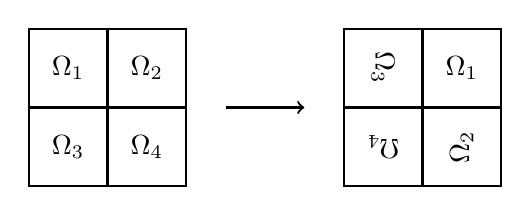
\begin{tikzpicture}
    % Original Grid
    \draw[thick] (0,0) rectangle (2,2);
    \draw[thick] (1,0) -- (1,2);
    \draw[thick] (0,1) -- (2,1);

    \node at (0.5,1.5) {$\Omega_1$};
    \node at (1.5,1.5) {$\Omega_2$};
    \node at (0.5,0.5) {$\Omega_3$};
    \node at (1.5,0.5) {$\Omega_4$};

    % Arrow
    \draw[->, thick] (2.5,1) -- (3.5,1);

    % Transformed Grid
    \begin{scope}[shift={(4,0)}]
        \draw[thick] (0,0) rectangle (2,2);
        \draw[thick] (1,0) -- (1,2);
        \draw[thick] (0,1) -- (2,1);

        \node at (0.5,1.5) {\rotatebox{270}{$\Omega_3$}}; % Rotated 180° horizontally
        \node at (1.5,1.5) {$\Omega_1$};             % No change
        \node at (0.5,0.5) {\rotatebox{180}{$\Omega_4$}}; % Upside down
        \node at (1.5,0.5) {\rotatebox{90}{$\Omega_2$}};  % 90° rotation
    \end{scope}
\end{tikzpicture}
\caption{Maišymo transformacijos pavyzdys}
\end{figure}

\begin{figure}[h]
    \centering
    \begin{minipage}[c]{0.40\textwidth}
        \centering
        \includegraphics[width=\textwidth]{images/rnd-mix-left-c0-1.png}\\
        \includegraphics[width=\textwidth]{images/rnd-mix-left-c1-1.png}\\
        \includegraphics[width=\textwidth]{images/rnd-mix-left-c2-1.png}
    \end{minipage}%
    \hfill
    \begin{minipage}[c]{0.1\textwidth}
        \centering
        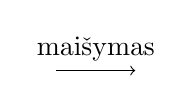
\begin{tikzpicture}
            \draw[->] (0,0.5) -- (1,0.5);
            \node[above] at (0.5, 0.5) {maišymas};
        \end{tikzpicture}
    \end{minipage}%
    \hfill
    \begin{minipage}[c]{0.45\textwidth}
        \centering
        \includegraphics[width=\textwidth]{images/rnd-mix-right-c0-1.png}\\
        \includegraphics[width=\textwidth]{images/rnd-mix-right-c1-1.png}\\
        \includegraphics[width=\textwidth]{images/rnd-mix-right-c2-1.png}
    \end{minipage}

    \caption{Atsitiktinis maišymo modelis pritaikytas skaitiniame modelyje. Maišymo laikas $t^1_\text{mix} = 1\text{h}\,30\text{min}$ }

    \label{fig:random-mix-example}

\end{figure}

\ref{fig:random-mix-example}-ame pavyzdyje matome kaip atrodo reakcijos eiga, kada vyksta išmaišymas. Trečiame stulpelyje ir ypatingai trečios medžiagos koncentracijoje matome ryškių artefaktų. Taip yra todėl, kad nuo išmaišymo praejo labai mažai laiko ir medžiagos nespėjo sureaguoti naujoje aplinkoje. Tarp laiko momentų $t=1h\,30min$ ir $t=5h\,59min$ trečios medžiagos $c_3$ koncentracija daugiausiai keitėsi tose vietose, kuriose iš pradžių vyko reakcija, tačiau galime matyti ir visiškai naujos sienelės susidaryma ties srities viduriu. Norint geriau suprasti kokį poveikį toks išmaišymas turi reakcijos pabaigos lakui reikėtų ištirti trečios medžiagos koncentracijos priklausomybę nuo laiko.

\newpage
\begin{figure}[h!]
    \centering
    \includegraphics[width=0.45\textwidth]{images/bad-mix-qnt-1.png}
    \caption{Kompiuterinio modelio rezultatų palyginimas, kai išmaišymas vyksta ir nevyksta.  }
    \label{bad-mix-qnt-example}
\end{figure}
\ref{bad-mix-qnt-example}-ame pavyzdyje puikiai matosi, kad išmaišymas nepagreitino reakcijos, o ją sulėtino. Reakcijos laikas su išmaišymu yra apytiksliai dvejom su puse valandom ilgesnis. Ši problema atsiranda todėl, kad mes modeliuojame ypač mažą reakcijos erdvės sritį, kurioje susiduria tik 4 mikrodalelės, dėl to nėra daug skirtingų išdėstymų, kada viena sienele galėtų dalintis skirtingų medžiagų dalelės, prie to žinoma prisideda ir faktas, kad šis modelis yra dviejų dimensijų. Eksperimentas parodė, kad nesuveiktų ir statistinis bandymas - vidutinis atsitiktinis išmaišymas taip pat neduoda geresnių rezultatų negu reakcijos modelis be išmaišymų. Dėl šios priežasties apsvarstysime alternatyvų išmaišymo metoda.

\subsection{Tobulas maišymas}

Kad išspręstume atsitiktinio maišymo problemą, modeliuosime tobulą teorinį išmaišymą, kuris turės didžiausią poveikį reakcijos greičiui. Pats maišymo modelis išliks toks pat, tačiau sritis $\Omega_i$ sudėliosime ne atsitiktinai, o sukeisime įstrižai. Tobulas išmaišymas aišku priklauso nuo pradinių sąlygų, o šis galioja tik duotoms pradinėms sąlygoms \eqref{intial-cond}.

\begin{figure}[!h]
\centering
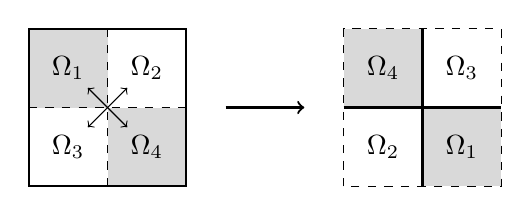
\begin{tikzpicture}
    % Original Grid
    \fill[gray!30] (0,1) rectangle (1, 2);
    \fill[gray!30] (1,0) rectangle (2, 1);
    \draw[<->] (0.75,0.75) -- (1.25,1.25);
    \draw[<->] (1.25,0.75) -- (0.75,1.25);
    \draw[thick] (0,0) rectangle (2,2);
    \draw[dashed] (1,0) -- (1,2);
    \draw[dashed] (0,1) -- (2,1);

    \node at (0.5,1.5) {$\Omega_1$};
    \node at (1.5,1.5) {$\Omega_2$};
    \node at (0.5,0.5) {$\Omega_3$};
    \node at (1.5,0.5) {$\Omega_4$};

    % Arrow
    \draw[->, thick] (2.5,1) -- (3.5,1);

    % Transformed Grid
    \begin{scope}[shift={(4,0)}]
        \fill[gray!30] (0,1) rectangle (1, 2);
        \fill[gray!30] (1,0) rectangle (2, 1);
        
        \draw[dashed] (0,0) rectangle (2,2);
        \draw[thick] (1,0) -- (1,2);
        \draw[thick] (0,1) -- (2,1);

        \node at (0.5,1.5) {$\Omega_4$};
        \node at (1.5,1.5) {$\Omega_3$};
        \node at (0.5,0.5) {$\Omega_2$};
        \node at (1.5,0.5) {$\Omega_1$};
    \end{scope}
\end{tikzpicture}
\caption{Tobulo maišymo transformacija}
\label{perfect-2x2-mix}
\end{figure}
\ref{perfect-2x2-mix}-ame pavyzdyje matoma prieš tai apibūdintą transformacija. Punktyrinės linijos kairėje pusėje žymi sieneles ties kuriomis vyksta reakcija. Šiuo atveju po išmaišymo nėra sričių, kurios turėtų bendrą punktyrinę sienelę, o tai reiškia, kad tokiu būdu sumaišius sritis, visos vidinės sienelės turės didžiausią įmanomą skirtingų medžiagų kontrastą, kuris lems didžiausią įmanomą reakcijos pagreitėjimą.

\subsubsection*{Tobulo maišymo rezultatai}

\begin{figure}[h!]
  \centering
  \includegraphics[width=0.75\textwidth]{images/mixing/perfect-mix-ord-0-c1.png} \\ 
  \includegraphics[width=0.75\textwidth]{images/mixing/perfect-mix-ord-0-c3.png}
  \caption{Tobulo maišymo poveikis skaitiniame sprendinyje. Modelio parametrai atitinka reakciją vykstančia $1000\degree C$ temperatūroje. Modeliuojamos srities rezoliucija $40\times40$. Išmaišymo laikas -- $1\text{h}. $}
  \label{fig:perfect-mix-small-example}
\end{figure}

\ref{fig:perfect-mix-small-example}-ame pavyzdyje matome kaip tobulas maišymo procesas paveikia reakcijos erdvę. Kaip ir su atsitiktinio maišymo modelio atveju, kokybiniai maišymo modelio rezultatai nėra pastebimi iš tokio reakcijos erdvės vaizdavimo, todėl analizuosime medžiagos kiekio priklausomybę nuo laiko.

\newpage

\begin{figure}[h!]
    \centering
    \includegraphics[width=0.5\textwidth]{../paper/images/mixing/perfect-mix-vs-no-mix-ord-0-q3.png}

    \caption{Kompiuterinio modelio rezultatų palyginimas tarp reakcijos be išmaišymo ir reakcijos su tobulu išmaišymu.  }

    \label{optimal-mix-qnt}
\end{figure}

Šiuo atveju, \ref{optimal-mix-qnt}-ame pavyzdyje matome, kad dėl tobulo išmaišymo galime matyti šuolį medžiagos kiekyje. Toks maišymas turi teigiamą poveikį reakcijos pabaigos laikui ir labiau atitinka eksperimentinius rezultatus negu atsitiktinis išmaišymas.
Čia galime pasamprotauti, kaip reakcijos pabaigos laikas priklauso nuo išmaišymo laiko - jei išmaišome pradinę konfigūraciją pačioje reakcijos pradžioje, rezultatams tai neturės jokios įtakos ir gausime reakcijos modelį be išmaišymo. Lygiai tas pats nutiktų jei išmaišymas įvyktų ką tik prieš reakcijos pabaigą, tačiau išmaišymas kitais laiko momentais, kaip jau matėme, gali sutrumpinti reakcijos pabaigos laiką. Jei pavaizduotume reakcijos trukmės priklausomybę nuo išmaišymo momento, gautume štai tokį grafiką:

\begin{figure}[h!]
    \centering
    \includegraphics[width=0.5\textwidth]{../paper/images/mixing/duration-mix-moment-dependance-ord0.png}

    \caption{Reakcijos trukmės priklausomybė nuo išmaišymo momento. Modelio parametrai atitinka reakciją $1000\degree C$ temperatūroje. Modeliuojamos srities rezoliucija $40\times40$. }

    \label{fig:duration-mix-moment-graph-for-small-space}
\end{figure}

\ref{fig:duration-mix-moment-graph-for-small-space}-ame pavyzdyje matome, kad priklausomybė nėra simetriška, reakcijos pabaigos laikas, kai išmaišymas nevyksta, yra apie 12val. Optimalus išmaišymo laikas yra apie 40min ir tokiu atveju 97\% medžiagų sureaguos per 11h 7min.

\newpage

\subsection{Reakcijos modeliavimas didesnėje srityje}

Modeliuoti mažą visos reakcijos erdvės sritį užtenka norint gauti tikslias aproksimacijas difuzijos bei reakcijos greičio konstantoms \cite{mackeviciusCloserLookComputer2012}. Tačiau modeliuodami medžiagų išmaišymą neturime priežasties daryti tokios pačios prielaidos. Norint modeliuoti didesnę erdvės sritį, pradines sąlygas reikia atkartoti veidrodiniu principu, tuo galima įsitikinti pažvelgus į \ref{fig:periodic-space}-ą pavyzdį. Modeliuojant didesnę erdvę, ne tik padidės srities plotas, kaip pavaizduota \ref{large-initial-conditions}-ame pavyzdyje, tačiau ir padvigubinsime diskrečių taškų kiekį kiekviena erdvine kryptimi. Šį procesą galima rekursyviai kartoti ir tokiu būdu gauti eksponentiškai didesnės srities pradines sąlygas.


\begin{figure}[h!]
\centering
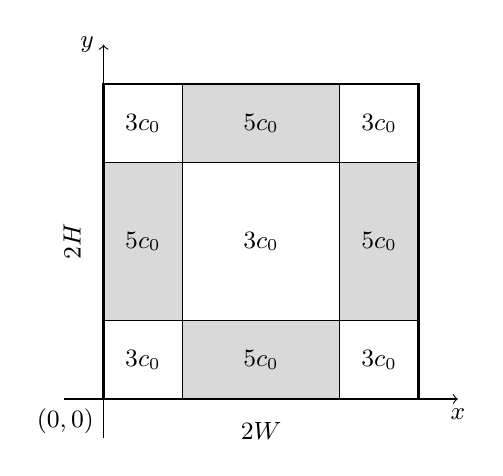
\begin{tikzpicture}
  
    % Fill the boundary cells
    % \fill[gray!30] (0, 3) rectangle (1, 4); % Top-left
    \fill[gray!30] (1, 3) rectangle (3, 4); % Top
    % \fill[gray!30] (3, 3) rectangle (4, 4); % Top-right
    \fill[gray!30] (0, 1) rectangle (1, 3); % Left
    \fill[gray!30] (3, 1) rectangle (4, 3); % Right
    % \fill[gray!30] (0, 0) rectangle (1, 1); % Bottom-left
    \fill[gray!30] (1, 0) rectangle (3, 1); % Bottom
    % \fill[gray!30] (3, 0) rectangle (4, 1); % Bottom-right

    % Draw the outer rectangle
    \draw[thick] (0, 0) rectangle (4, 4);
    \node at (2, -0.4) {\small $2W$};
    \node[rotate=90] at (-0.4, 2) {\small $2H$};

    % Draw the inner rectangle
    \draw[-] (0, 1) -- (4, 1);
    \draw[-] (0, 3) -- (4, 3);
    \draw[-] (1, 0) -- (1, 4);
    \draw[-] (3, 0) -- (3, 4);

    % Labels
    \node at (0.5, 3.5) {\small $3c_0$};
    \node at (2, 3.5) {\small $5c_0$};
    \node at (3.5, 3.5) {\small $3c_0$};

    \node at (0.5, 2) {\small $5c_0$};
    \node at (2, 2) {\small $3c_0$};
    \node at (3.5, 2) {\small $5c_0$};

    \node at (0.5, 0.5) {\small $3c_0$};
    \node at (2, 0.5) {\small $5c_0$};
    \node at (3.5, 0.5) {\small $3c_0$};

    % Coordinate axes
    \draw[->] (-0.5, 0) -- (4.5, 0) node[anchor=north] {\small $x$};
    \draw[->] (0, -0.5) -- (0, 4.5) node[anchor=east] {\small $y$};
    \node[anchor=north east] at (0, 0) {\small $(0,0)$};
\end{tikzpicture}
\caption{Keturis kartus padidinta pradinių sąlygų sritis. }

\label{large-initial-conditions}
\end{figure}

\subsection{Maišymo modelių pritaikymas didesnėms sritims}

\subsubsection*{Atsitiktinis maišymas}

Praplėsti atsitiktinį maišymo modelį didesnei sričiai yra trivialu -- sugeneruojame $N^2\text{-permutaciją}$ ir $N^2$ atsitiktinių kampų $\theta_1, \theta_2, \dots, \theta_{N^2}$, kur $N$ yra sričių skaičius didesnėje erdvėje. Tuomet maišymo metu, kiekvieną sritis įgauna nauja poziciją bei posukio kampą.

\subsubsection*{Tobulas maišymas}

Tobulo maišymo modelį pritaikyti didesnėms sritims taip pat nėra sudėtinga -- tą galime padaryti atkartodami modelį veidrodžio principu:

\begin{figure}[!h]
\centering
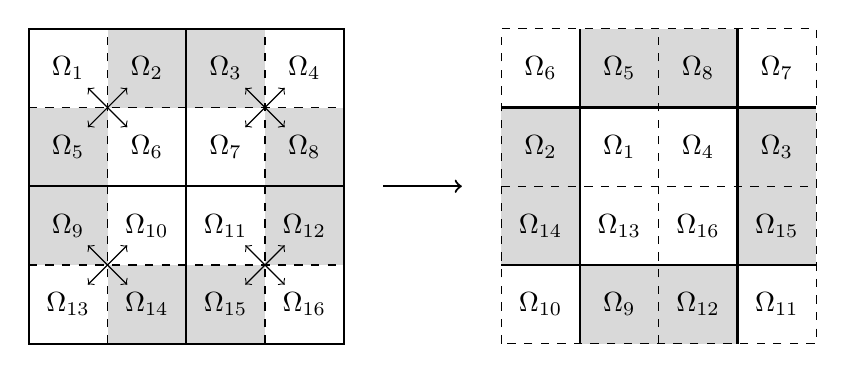
\begin{tikzpicture}
    % Original Grid

    \fill[gray!30] (1, 0) rectangle (3, 1);
    \fill[gray!30] (1, 3) rectangle (3, 4);

    \fill[gray!30] (0, 1) rectangle (1, 3);
    \fill[gray!30] (3, 1) rectangle (4, 3);

    \draw[thick] (0,0) rectangle (2,2);
    \draw[thick] (0,2) rectangle (2,4);
    \draw[thick] (2,0) rectangle (4,2);
    \draw[thick] (2,2) rectangle (4,4);
    \draw[dashed] (1,0) -- (1,4);
    \draw[dashed] (0,1) -- (4,1);
    \draw[dashed] (3,0) -- (3,4);
    \draw[dashed] (0,3) -- (4,3);

    \draw[<->] (0.75,0.75) -- (1.25,1.25);
    \draw[<->] (1.25,0.75) -- (0.75,1.25);

    \draw[<->] (2.75,0.75) -- (3.25,1.25);
    \draw[<->] (3.25,0.75) -- (2.75,1.25);

    \draw[<->] (0.75,2.75) -- (1.25,3.25);
    \draw[<->] (1.25,2.75) -- (0.75,3.25);

    \draw[<->] (2.75,2.75) -- (3.25,3.25);
    \draw[<->] (3.25,2.75) -- (2.75,3.25);

    \node at (0.5,3.5) {$\Omega_1$};
    \node at (1.5,3.5) {$\Omega_2$};
    \node at (0.5,2.5) {$\Omega_5$};
    \node at (1.5,2.5) {$\Omega_6$};

    \node at (2.5,3.5) {$\Omega_3$};
    \node at (3.5,3.5) {$\Omega_4$};
    \node at (2.5,2.5) {$\Omega_7$};
    \node at (3.5,2.5) {$\Omega_8$};

    \node at (0.5,1.5) {$\Omega_9$};
    \node at (1.5,1.5) {$\Omega_{10}$};
    \node at (0.5,0.5) {$\Omega_{13}$};
    \node at (1.5,0.5) {$\Omega_{14}$};

    \node at (2.5,1.5) {$\Omega_{11}$};
    \node at (3.5,1.5) {$\Omega_{12}$};
    \node at (2.5,0.5) {$\Omega_{15}$};
    \node at (3.5,0.5) {$\Omega_{16}$};

    % Arrow
    \draw[->, thick] (4.5,2) -- (5.5,2);

    % Transformed Grid
    \begin{scope}[shift={(6,0)}]
        \fill[gray!30] (1, 0) rectangle (3, 1);
        \fill[gray!30] (1, 3) rectangle (3, 4);

        \fill[gray!30] (0, 1) rectangle (1, 3);
        \fill[gray!30] (3, 1) rectangle (4, 3);

        \draw[dashed] (0,0) rectangle (4,4);

        \draw[dashed] (2,0) -- (2,4);
        \draw[dashed] (0,2) -- (4,2);

        \draw[thick] (1,0) -- (1,4);
        \draw[thick] (0,1) -- (4,1);
        \draw[thick] (3,0) -- (3,4);
        \draw[thick] (0,3) -- (4,3);

        \node at (0.5,3.5) {$\Omega_6$};
        \node at (1.5,3.5) {$\Omega_5$};
        \node at (0.5,2.5) {$\Omega_2$};
        \node at (1.5,2.5) {$\Omega_1$};

        \node at (2.5,3.5) {$\Omega_8$};
        \node at (3.5,3.5) {$\Omega_7$};
        \node at (2.5,2.5) {$\Omega_4$};
        \node at (3.5,2.5) {$\Omega_3$};

        \node at (0.5,1.5) {$\Omega_{14}$};
        \node at (1.5,1.5) {$\Omega_{13}$};
        \node at (0.5,0.5) {$\Omega_{10}$};
        \node at (1.5,0.5) {$\Omega_{9}$};

        \node at (2.5,1.5) {$\Omega_{16}$};
        \node at (3.5,1.5) {$\Omega_{15}$};
        \node at (2.5,0.5) {$\Omega_{12}$};
        \node at (3.5,0.5) {$\Omega_{11}$};
    \end{scope}
\end{tikzpicture}
\caption{Tobulo maišymo transformacija ant keturis kartus padidintų pradinių sąlygų}
\label{perfect-4x4-mix}
\end{figure}
\ref{perfect-4x4-mix}-ame pavyzdyje matome kaip atrodo tobulas išmaišymas praplėstų pradinių sąlygų atveju. Punktyrinės linijos žymi skirtingų medžiagų bendras sieneles t. y. tas sieneles, ties kuriomis aktyviai vyksta medžiagų reakcija. Paprastos linijos žymi sieneles, ties kuriomis susiduria tos pačios medžiagos sritys arba sieneles, kurios yra nukreiptos į išorę. Toks išmaišymas žymiai padidina reakcijos greitį todėl, kad visos sienelės tarp skirtingų medžiagų yra dar nesureagavusios ir turi didelį koncentracijų kontrastą.
\subsection{Modelio rezultatai didesnėse srityse}
Norint modeliuoti maišymą ir tirti šio proceso savybes skirtingo dydžio srityse turime atsižvelgti į tai, kad reakcijos modeliavimas skirtingo dydžio srityse be išmaišymo proceso gali suteikti nenuoseklius rezultatus, todėl pirmiausia turime išsiaiškinti esminius skirtumus tarp šių modelių. Viena svarbiausių modelio rezultatų savybių, kurias mes norėtume tirti yra reakcijos trukmė, todėl pažvelgsime kaip ji kinta priklausomai nuo srities dydžio kurią modeliuojame. Kaip aprašėme praeituose skyriuose, pradinę reakcijos sritį mes galime didinti keturis kartus ir tai daryti rekursyviai, todėl mūsų modeliuojamos sritys didės eksponentiškai.
\begin{figure}[h!]
    \centering
    \includegraphics[width=0.5\textwidth]{images/mixing/duration-order-T1000.png}

    \caption{Reakcijos trukmės priklausomybė nuo to, kiek kartų buvo padidintos pradinės sąlygos \eqref{fig:initial-condition-visual}. }

    \label{fig:duration-order-dependance}
\end{figure}
\subsection{Atsitiktinis maišymas didesnėse srityse}
\ref{fig:random-mix-larger-example}-ame pavyzdyje matome kaip atrodo atsitiktinis išmaišymas skaitiniame sprendinyje. Svarbu atkreipti dėmesį į tai, kad sumaišius sritis niekada neatsiras sričių, kuriose skirtingų medžiagų koncentracijos žymiai persidengia, taip yra todėl, kad vykstant maišymui visos tam tikroje srityje esančios medžiagos bus transformuotos tokiu pat būdu, o kadangi pradinėse sąlygose medžiagos nepersidengia -- išmaišytos medžiagos taip pat nepersidengs. Idealus rezultatas, kurio galime tikėtis atlikus atsitiktinį maišymą yra alternuojantis sričių išsidėstymas pagal koncentraciją kaip šachmatų lentoje -- tokiu būdu, difuzijos pagalba, skirtingas medžiagas laikančios sritys viena kitą galės pasiekti greičiausiai.

\newpage

\begin{figure}[h!]
  \centering
  \includegraphics[width=0.75\textwidth]{images/mixing/random-mix-ord-1-c1.png} \\ 
  \includegraphics[width=0.75\textwidth]{images/mixing/random-mix-ord-1-c2.png} \\
  \includegraphics[width=0.75\textwidth]{images/mixing/random-mix-ord-1-c3.png}
  \caption{Atsitiktinio maišymo poveikis skaitiniam sprendiniui. Modeliuojama sritis padidinta 4 kartus. Modelio parametrai atitinka reakciją vykstančia $1000\degree C$ temperatūroje. Modeliuojamos srities rezoliucija $80\times80$. Išmaišymo laikas -- $1\text{h}. $}
  \label{fig:random-mix-larger-example}
\end{figure}

Problema su kuria susidūrėme modeliuodami pačią mažiausią erdvės sritį išlieka ir čia -- erdvė per maža, kad išmaišymas sutrumpintų reakcijos laiką. Šiuo atveju nebūtų praktiška pateikti reakcijos trukmės nuo išmaišymo momento priklausomybės grafiką todėl, kad kiekvienam išmaišymo momentui reikėtų rasti kelis sprendinius. Vis dėl to galime pabandyti pasinaudoti pastebėjimu, kad optimalus išmaišymo laikas tobulo maišymo atveju yra apie 40min ir pabandyti ištirti kaip atsitiktinis maišymas paveikia reakcijos trukmę, kai maišymą atliekame šiuo, optimaliu momentu. 

\begin{figure}[h!]
  \centering
  \includegraphics[width=\textwidth]{images/mixing/sample-durations-random-mix.png}
  \caption{Vidutinės reakcijos trukmės skirtingo dydžio erdvėse, kai modeliuojamas atsitiktinis išmaišymas. Kiekvienam pavaizduotam srities dydžiui buvo padaryta 20 individualių sprendinių (bandymų) su atsitiktiniu išmaišymu. Išmaišymo laikas -- 40min. Pavaizduotas individualių sprendinių reakcijos trukmės laikas bei jų vidurkis.}
  \label{fig:random-samples}
\end{figure}

Pavyzdyje~\ref{fig:random-samples} matyti, kad erdvės didinimas daro neigiamą įtaką reakcijos trukmei: kuo didesnė modeliuojama erdvė, tuo ilgesnė vidutinė reakcijos trukmė. Manome, kad tokie rezultatai gaunami todėl, jog net ir padidinus erdvę 64 kartus, nesusidaro pakankamos sąlygos, leidžiančios atsitiktiniam maišymui paspartinti reakciją. Be to, veidrodiniu principu atkartotos pradinės sąlygos iš karto sukuria pakankamai palankų sričių išsidėstymą visoje reakcijos erdvėje, kurį atsitiktinis išmaišymas kaip tik suardo.

\subsection{Tobulo maišymo rezultatai didesnėse srityse}

\begin{figure}[h!]
  \centering
  \includegraphics[width=0.75\textwidth]{images/mixing/perfect-mix-ord-1-c1.png} \\ 
  \includegraphics[width=0.75\textwidth]{images/mixing/perfect-mix-ord-1-c2.png} \\
  \includegraphics[width=0.75\textwidth]{images/mixing/perfect-mix-ord-1-c3.png}
  \caption{Tobulo maišymo poveikis skaitiniam sprendiniui. Modeliuojama sritis padidinta 4 kartus. Modelio parametrai atitinka reakciją vykstančia $1000\degree C$ temperatūroje. Modeliuojamos srities rezoliucija $80\times80$. Išmaišymo laikas -- $1\text{h}. $}
  \label{fig:perfect-mix-larger-example}
\end{figure}



Viena iš pageidautinų maišymo modelių savybių -- nuoseklus rezultatai, kurie būtų nepriklausomi nuo srities dydžio, kurią modeliuojame. Tokiu atveju, galėtume daryti reikšmingas išvadas apie maišymo poveikį reakcijai modeliuojant mažas sritis lyginant su tikra reakcija. Norint patikrinti ar tobulo maišymo modelis pasižymi šia savybe, pirmiausia galime palyginti kaip 


\sectionnonum{Rezultatai ir išvados}

\subsection*{Rezultatai}

Šiame darbe buvo įgyvendinti šie uždaviniai:

\begin{itemize}
    \item Sudaryti kompiuteriniai YAG reakcijos modeliai remiantis išreikštiniu ir ADI skaitiniais metodais. 
    \item Teoriškai parodyta išreikštinio skaitinio modelio stabilumo sąlyga
    \item Sukurta kintamo laiko žingsnio strategija, kuri leidžia efektyviai modeliuoti YAG sintezės reakciją didelėse srityse
    \item Išreikštinio modelio rezultatai buvo verifikuojami ir buvo užtikrinta, kad modelis veikia korektiškai 
    \item Abu skaitiniai modeliai buvo analizuojami, išmatuotas jų efektyvumas bei tikslumas
    \item Atsitiktinio ir tobulo maišymo modeliai integruoti į kompiuterinius (YAG) reakcijos modelius
    \item Ištirtas maišymo modelių poveikis įvairaus dydžio erdvėse 
\end{itemize}

\subsection*{Išvados}

Iš rezultatų analizės galima daryti šias išvadas:

\begin{itemize}
    
    \item Modeliuojant tobulą išmaišymą YAG reakcijoje, optimalus maišymo laikas nepriklauso nuo modeliuojamos srities dydžio.

    \item Modeliuojant tobulą išmaišymą YAG reakcijoje, optimali reakcijos trukmė konverguoja didinant modeliuojamą sritį.

    \item Tobulo maišymo modelis atspindi savybes, kuriomis pasižymi realus maišymo procesas. Jei maišymas vyksta reakcijos pradžioje arba pabaigoje nepastebime jokio pokyčio reakcijos trukmėje, tačiau maišant kitais laiko momentais pastebime, kad reakcijos trukmė trumpėja.

    \item Kintamo laiko žingsnio strategija leidžia ypač efektyviai spręsti YAG reakcijos uždavinį, o įtaka sprendinio tikslumui yra nereikšminga.

    \item Atsitiktinis maišymo modeliavimas neturi savybių, kuriomis turėtų pasižymėti bet koks maišymo modelis -- beveik visuomet reakcijos trukmė pailgėja. Tai galioja tada, kai modeliuojama erdvė yra dviejų dimensijų ir yra nedidelė palyginus su tikraja reakcijos erdve. Rezultatai rodo, kad net 64 kartus padidintoje srityje (originali sritis yra vienos mikrodalelės dydžio) vidutinis reakcijos laikas pailgėja daugiau nei 40 valandų, todėl laikome, kad atsitiktinis maišymo modelis yra nepraktiškas.

\end{itemize}

\printbibliography[title = {Literatūra ir šaltiniai}]

\end{document}